\pdfoutput=1
\documentclass[11pt]{amsart}
\usepackage{amsmath,amssymb,amsthm}
\usepackage[margin=1.2in]{geometry}
\usepackage{booktabs,adjustbox,graphicx}
\usepackage{xcolor,tikz}
\usetikzlibrary{arrows.meta,calc,positioning}
\usepackage[colorlinks=true,linkcolor=blue,citecolor=blue,urlcolor=blue]{hyperref}
\hypersetup{pdfauthor={Bernd Johannes Wuebben},
 pdftitle={Exceptional cycles and harmonic metrics in K3 bundle moduli}}
\setlength{\emergencystretch}{2em}
\newtheorem{theorem}{Theorem}[section]
\newtheorem{proposition}[theorem]{Proposition}
\newtheorem{lemma}[theorem]{Lemma}
\newtheorem{corollary}[theorem]{Corollary}
\theoremstyle{definition}
\newtheorem{definition}[theorem]{Definition}
\newtheorem{example}[theorem]{Example}
\theoremstyle{remark}
\newtheorem{remark}[theorem]{Remark}
\newcommand{\Z}{\mathbb Z}
\newcommand{\R}{\mathbb R}
\newcommand{\C}{\mathbb C}
\newcommand{\PP}{\mathbb P}
\newcommand{\FF}{\mathbb F}
\newcommand{\OO}{\mathcal O}
\newcommand{\cE}{\mathcal E}
\newcommand{\Q}{\mathcal Q}
\newcommand{\ddbar}{\bar\partial}
\newcommand{\NS}{\operatorname{NS}}
\newcommand{\Ext}{\operatorname{Ext}}
\newcommand{\Hom}{\operatorname{Hom}}
\newcommand{\End}{\operatorname{End}}
\newcommand{\Aut}{\operatorname{Aut}}
\newcommand{\tr}{\operatorname{tr}}
\newcommand{\rank}{\operatorname{rank}}
\newcommand{\im}{\operatorname{im}}
\newcommand{\Vol}{\operatorname{Vol}}
\newcommand{\diam}{\operatorname{diam}}
\newcommand{\coker}{\operatorname{coker}}
\newcommand{\Gr}{\operatorname{Gr}}
\newcommand{\Lie}{\operatorname{Lie}}
\title[Exceptional cycles and harmonic metrics]{Exceptional cycles and harmonic metrics\\ in K3 bundle moduli}
\author{Bernd Johannes Wuebben}
\subjclass[2020]{14J60 (primary); 14J28, 53C26, 53C07 (secondary)}
\keywords{K3 surface, moduli of bundles, stability wall, exceptional cycle,
 harmonic metric, integral cohomology, hyperk\"ahler quotient}
\date{November 7, 2026}


\begin{document}
\begin{abstract}
We construct compact moduli fourfolds of bundles on a K3 surface whose
common contraction has a singular surface and one deeper point. In a specified
stability chamber, a moving projective line specializes with multiplicity
one to a line in each of two Lagrangian planes. We identify the primitive
integral curve and surface classes and calculate their intersection
matrix. Restriction from the complement to the boundary of a neighborhood
of the planes gives an explicit congruence modulo eight determining their
degree-four integral cohomological gluing. For the natural $L^2$ metric
on moduli, defined by harmonic deformation representatives, these same
cycles have exact areas and volumes and ambient diameter estimates uniform
as the two positive stability parameters vanish at unrelated rates. At separated
scales, rescalings based on the smaller plane converge in pointed
Gromov--Hausdorff topology to the complete Calabi metric on $T^*\PP^2$.
The central harmonic metric completes to the common contraction, which
is the compact Gromov--Hausdorff limit of the chamber spaces. The proof
combines a complete boundary analysis with convergent
symplectic coordinates and relative harmonic estimates. An isolated-plane
contraction provides the corresponding congruence modulo three.
\end{abstract}
\maketitle
\section{Introduction}\label{sec:introduction}

A stability wall can contract a family of curves and a higher-dimensional
exceptional fibre at the same time. The topology of the smooth moduli
space then depends on how these cycles meet, while its metric degeneration
depends on the relative rates at which their periods vanish. The two
questions concern the same geometric objects. To relate them, a local
description of a singularity must be placed inside a compact moduli
problem, with its full boundary and its actual harmonic metric.

We carry this out for two explicit moduli problems on K3 surfaces. The
first contracts one Lagrangian plane. The second has a moving family of
projective lines and a deeper fibre consisting, in one chamber, of two
Lagrangian planes meeting at a point. A moving line degenerates into one
line in each plane. This specialization gives an integral relation among
global curve classes and an exact identity among their harmonic areas.
The intersection of the planes also changes the integral attachment:
the relevant boundary group is cyclic of order eight, whereas the
boundary of a single plane has order three.

\subsection{The compact family}
For a sheaf on a K3 surface, use the Mukai vector and pairing
\[
 v(F)=(r,c_1,r+c_1^2/2-c_2),\qquad
 (r,c,s)\cdot(r',c',s')=c\cdot c'-rs'-r's.
\]
Choose a K3 surface $X$ with full N\'eron--Severi lattice generated by
$H,D_1,D_2$, where $H$ is ample and the intersection matrix is
\begin{equation}\label{eq:intro-lattice}
 \begin{pmatrix}2&0&0\\0&-6&-4\\0&-4&-8\end{pmatrix}.
\end{equation}
Such a surface exists by the construction in
Section~\ref{sec:compact-interaction}. Put
\[
 L_0=\OO_X,\quad L_1=\OO_X(D_1),\quad L_2=\OO_X(D_2),
 \qquad a_i=v(L_i),\qquad v=a_0+a_1+a_2.
\]
Thus $v=(3,D_1+D_2,-4)$ and $v^2=2$. Let $\omega_\eta$ be the
Ricci-flat representative of $H+sD_1+tD_2$, for
$\eta=(s,t)$ near zero. The normalized stability parameters are
\begin{equation}\label{eq:intro-levels}
 \zeta(\eta)=\frac{2\pi}{3}
 \begin{pmatrix}-10&-12\\8&0\\2&12\end{pmatrix}
 \binom{s}{t},\qquad \zeta_0+\zeta_1+\zeta_2=0.
\end{equation}
The three lines $\zeta_i=0$ divide the parameter plane into six
chambers. By a generic parameter below we mean a point outside these
lines in a sufficiently small neighborhood of the origin.

On a smooth moduli space we use the real part of the unnormalized
Dolbeault harmonic $L^2$ pairing, at fixed holomorphic determinant.
Write $g_\eta$ for this metric and $\Omega_\eta$ for its K\"ahler
form. All distances between exceptional points are measured in the
entire moduli space. Integral cohomology is understood unless another
coefficient group is displayed.

\begin{theorem}\label{thm:main}
For the family above, the following assertions hold.
\begin{enumerate}
\item Each generic chamber $\sigma$ has a smooth compact projective
moduli fourfold $M_\sigma$ of slope-stable bundles, of deformation
type $X^{[2]}$. There are projective symplectic contractions
$\pi_\sigma:M_\sigma\to Z$ to a common normal projective fourfold.
The regular locus of $Z$ is the moduli of $H$-stable bundles. Its
reduced singular locus is a normal K3 surface $T$ with one $A_1$ point $o$.
The fibres over $T\setminus\{o\}$ are projective lines. Over $o$
the fibre is two planes meeting transversely at a point in the
chambers with signs $(+,-,+)$ and $(-,+,-)$; in the other four
chambers it is $\PP^2\cup\FF_1$, meeting along a line and the
negative section. Every central or nearby ideal HYM object has zero
lost charge, and every sheaf in these moduli problems is locally free.

\item Fix $\zeta_0=a>0$, $\zeta_2=b>0$ and
$\zeta_1=-a-b$. Write $P_0,P_2$ for the two planes, $c_0,c_2$
for their line classes, and $f$ for a moving fibre class. These
classes satisfy
\begin{equation}\label{eq:intro-specialization}
 f=c_0+c_2,
 \qquad
 \left(\int_{M_\sigma}[P_i][P_j]\right)_{i,j=0,2}
   =\begin{pmatrix}3&1\\1&3\end{pmatrix}.
\end{equation}
The curve and surface pairs each span a primitive rank-two integral
subgroup. A proper flat analytic family realizes the curve relation
with both multiplicities equal to one. For
$V=M_\sigma\setminus(P_0\cup P_2)$, let $L$ be the boundary of
a regular neighborhood of the planes. Then $H^4(L)=\Z/8$, and
restriction to $L$ is an explicit surjection
$\kappa:H^4(V)\to\Z/8$ such that restriction identifies
\begin{equation}\label{eq:intro-attachment}
 H^4(M_\sigma)=
 \{(u,n_0,n_2)\in H^4(V)\oplus\Z^2:
       n_0-3n_2\equiv\kappa(u)\pmod 8\}.
\end{equation}
Proposition~\ref{prop:calculated-attachments} evaluates the map on
Chern classes of family indices associated with a universal bundle.
The complement cohomology ring, together with these distinguished
restricted classes, is retained global data.

\item The same cycles have exact harmonic areas and volumes
\begin{equation}\label{eq:intro-volumes}
 \begin{gathered}
 \operatorname{Area}(c_0)=\pi a,\qquad
 \operatorname{Area}(c_2)=\pi b,\qquad
 \operatorname{Area}(f)=\pi(a+b),\\
 \Vol(P_0)=\frac{\pi^2a^2}{2},\qquad
 \Vol(P_2)=\frac{\pi^2b^2}{2}.
 \end{gathered}
\end{equation}
Their ambient diameters are comparable to $\sqrt a$ and $\sqrt b$,
with constants independent of $a/b$. As $a/b\to0$ and
$a+b\to0$, rescaling distances by $a^{-1/2}$ at $P_0$ gives the
complete unit-level Calabi quotient on $T^*\PP^2$, and
\[
 \frac{\diam_{M_\sigma}P_0}{\sqrt a}\longrightarrow\frac\pi2.
\]
The reversed hierarchy has the corresponding conclusion for $P_2$.
There are also complete successive pointed limits at any fixed finite
number of scales, under the convergence hypotheses on normalized
levels and normal basepoints in Theorem~\ref{thm:successive-limits}.
The harmonic metric on $Z_{\rm reg}$ has compact completion
$(Z,d_0)$ with its projective topology, and
\[
 (M_{\sigma(\eta)},g_\eta)\longrightarrow(Z,d_0)
 \quad\text{in compact Gromov--Hausdorff distance}
\]
along every generic sequence $\eta\to0$.
\end{enumerate}
\end{theorem}

The formula \eqref{eq:intro-attachment} records an integral additive
attachment. Its order-eight congruence depends on the intersection
of the two planes. It does not follow from the ranks of their
cohomology groups. The complement $V$ still contains the exceptional
geometry over the moving stratum; it differs from the common stable
open set. Section~\ref{sec:projective-family} describes that geometry
and computes its ring over the open stratum, retaining the nonzero
algebraic Brauer class of its projective-line bundle.

\subsection{A single plane and the proof mechanism}
Section~\ref{sec:isolated-plane} begins with the lattice
$\NS(X)=\Z H\oplus\Z D$, $H^2=2$, $H\cdot D=0$, $D^2=-22$,
and vector $(3,D,-4)$. The only strictly polystable central bundle
is $\OO_X\oplus B$, with $B$ a rigid rank-two bundle. Each adjacent
compact fourfold contracts a plane. Its primitive surface class has
square three, and the boundary of a normal neighborhood has fourth
cohomology $\Z/3$. The corresponding generator formula for the
attachment is the one-component version of
\eqref{eq:intro-attachment}. This example also fixes the metric
normalization: if $\kappa_t=44\pi|t|/3$, an exceptional line has
area $\pi\kappa_t$, and the plane has ambient diameter
$(\pi/2)\sqrt{\kappa_t}(1+O(|t|))$.

Three arguments connect these calculations to compact geometry.
First, an exhaustive rank calculation uses the lower bound $-2$ for
the Mukai square of a stable K3 sheaf to exclude every possible
lost-charge vector. Surface gauge compactness then applies without
concentration. Normalized inclusions and quotients in the central
Jordan--H\"older filtrations show that entire exceptional fibres
enter the local analytic charts. This supplies the global coverage
needed before a quotient model can identify a contraction.

Second, universal extension families determine restrictions of
integral classes to the exceptional cycles. These restrictions prove
primitivity and evaluate the boundary homomorphism. The family
$xy=t$ at the intersection of the two planes identifies the actual
specialization multiplicities. The two ingredients serve different
purposes: lattice pairings identify classes, while a proper flat
family proves their geometric specialization.

Third, the harmonic comparison is relative in every quotient
direction. Its error remains small even when one period is much
smaller than the other. A lower bound for the length required to
leave a chart then compares the two ambient distance infima. This
explains why the estimates apply to distances in the whole compact
moduli space, and why the rescaled limits are complete. Global
completion additionally uses the identification of the limiting
harmonic class with the ample class of the projective contraction.

\subsection{Relation to earlier work}
The existence and deformation type of the compact moduli spaces are
provided by Yoshioka's theorems \cite{yoshioka99,yoshioka01}. We use
the projective slope moduli of Greb--Toma \cite{grebtoma} and the
surface gauge comparison of Greb--Sibley--Toma--Wentworth
\cite{gstw}. Bayer--Macr\`i's theory \cite{bayermacri} supplies
the broader birational setting for stability walls. Local quiver
descriptions of K3 sheaf moduli are developed by Arbarello--Sacc\`a
\cite{arbarellosacca}. The two compact fibre configurations in
Theorem~\ref{thm:main} already occur in Bielawski--Dancer's
hypertoric examples \cite[Example~6.10]{bielawskidancer}; here they
are realized as the complete fibres of the stated compact
slope-moduli contractions.

Formality is also an established input to this subject.
Bandiera--Manetti--Meazzini \cite[Theorem~5.1]{bmm} prove DG-Lie
formality for coherent sheaves with linearly reductive automorphism
group on a smooth projective surface with trivial canonical bundle.
Their theorem applies to our common-slope direct sums. The related
projectively hyperholomorphic formality theorem is
\cite[Theorem~4.3]{meazzinionorati}. Section~\ref{sec:harmonic-models}
gives the additional coordinate information used for the metric
comparison: a convergent equivariant symplectic change whose first
correction is cubic. Relative finite balancing and the actual
harmonic reduction are the previously proved results
\cite{wuebben14,wuebben15}, restated below with the required
normalizations.

The plane-class identities and Hilbert-square cohomology are
classical \cite{hassetttschinkel,totaro,gottsche}; the calculation
here identifies their integral representatives and attachments in
the compact bundle-moduli problem. Markman's index generators
\cite{markman} make the attachment maps explicitly evaluable.
For the global metric completion we use Song \cite{song} and
Tosatti \cite{tosatti}, after checking their geometric and
metric hypotheses. The conclusions about cycle diameters and
successive scales have separate local proofs.

The resulting theorems concern exceptional cycles of compact
bundle-moduli contractions without bubbling. The complement and its
distinguished integral classes supply the global information retained
in the cohomological calculation.


\section{Convergent harmonic symplectic models}\label{sec:harmonic-models}

We first explain how the local equations and the metric use the same
coordinates. The qualitative quadraticity of the deformation problem
is known. The point needed here is control of the coordinate change
relative to the central harmonic norm.

\subsection{Conventions and the harmonic recursion}
Let $(X,\omega_0)$ be a Ricci-flat K3 surface and
\[
 E_0=\bigoplus_{i=1}^k F_i\otimes W_i
\]
a locally free slope-polystable bundle. The $F_i$ are pairwise
nonisomorphic stable bundles of common slope. Put $r_i=\rank F_i$
and $m_i=\dim W_i$, and choose a direct-sum Hermitian--Einstein
metric $h_0$. Write
\[
 d=\ddbar_{\End E_0},\quad V=H^1(X,\End E_0),\quad
 G=\prod_i\mathrm{GL}(W_i),\quad K=\prod_i\mathrm U(W_i).
\]
Ineffective factors are removed when taking effective quotients.
Since $H^1(X,\OO_X)=0$, all first-order deformations preserve the
holomorphic determinant. We use the $h_0,\omega_0$ harmonic norm.
Degrees are $c_1(F)\cdot[\omega]$, with no division by the volume
of $X$. The HE determinant connection varies with $\omega$.

Let $H_q$ and $G_q$ be the harmonic projections and Green operators.
At a fixed Sobolev order above the multiplication threshold, the
analytic implicit-function theorem solves
\begin{equation}\label{eq:harmonic-recursion}
 a(x)=x-d^*G_2(a(x)\wedge a(x)),\qquad
 F(x)=H_2(a(x)\wedge a(x))
\end{equation}
for small $x\in V$. Thus $a(x)=x+O(|x|^2)$, and $F=0$ is the
full convergent Kuranishi obstruction. The operators commute with
the parallel multiplicity matrices, so $a$ and $F$ are
$G$-equivariant wherever both sides are defined. This is a local
equivariance statement; a Euclidean ball is not $G$-invariant.

The surface hypothesis has a useful consequence. Since there are no
$(0,3)$-forms, $I-H_2=dd^*G_2$ on $(0,2)$-forms. Applying $d$ to
\eqref{eq:harmonic-recursion} gives the exact identity
\begin{equation}\label{eq:whole-curvature}
 da(x)+a(x)\wedge a(x)=F(x).
\end{equation}
It holds before imposing integrability. We will use it to regard the
obstruction itself as a moment map.

\subsection{A symplectic coordinate change with cubic correction}
Normalize the parallel holomorphic two-form $\sigma_X$ compatibly
with the harmonic norm, and define on $(0,1)$-forms
\[
 \mathcal B(\alpha,\beta)=
 \int_X\sigma_X\wedge\tr(\alpha\wedge\beta).
\]
In an adapted unitary coframe the antilinear operator
\begin{equation}\label{eq:quaternionic-J}
 J(A_1\bar\theta^1+A_2\bar\theta^2)
   =-A_2^*\bar\theta^1+A_1^*\bar\theta^2
\end{equation}
satisfies $J^2=-1$ and
$\mathcal B(\alpha,J\beta)=\langle\alpha,\beta\rangle_{L^2}$.
It preserves harmonic forms. Indeed the common-slope HE equation
makes the induced connection on $\End E_0$ anti-self-dual; the
K\"ahler identities, or integration by parts in the displayed
pairing followed by $J^2=-1$, give closedness and coclosedness of
$J\beta$ when $\beta$ is harmonic. This is the usual quaternionic
structure in the ASD moduli construction \cite{itoh}.

Let $B=a^*\mathcal B$ on $V$. It is closed and holomorphic.
Pairing curvature with a parallel endomorphism identifies its
complex moment with $F$, by \eqref{eq:whole-curvature} and Stokes'
theorem. For
$H_\xi(a)=\int_X\sigma_X\wedge\tr(\xi a\wedge a)$,
graded cyclicity of the trace gives
\[
 dH_\xi(a)(b)=\int_X\sigma_X\wedge
       \tr\bigl(\xi(b\wedge a+a\wedge b)\bigr)
       =\mathcal B([\xi,a],b).
\]
We use this convention for both the linear and nonlinear complex
moments.

The form $B_0$ is the Serre pairing on $V$. The correction
$D a_x-I$ takes values in $\im d^*$ and is $O(|x|)$. A harmonic
form is $\mathcal B$-orthogonal to $\im d^*$, by
\eqref{eq:quaternionic-J} and ordinary harmonic orthogonality.
The two terms linear in $Da_x-I$ therefore vanish, leaving
\begin{equation}\label{eq:symplectic-quadratic-error}
 B_x=B_0+O(|x|^2).
\end{equation}

\begin{proposition}\label{prop:symplectic-normal-form}
There is a $K$-equivariant holomorphic coordinate change on a
neighborhood of zero in $V$ such that
\begin{equation}\label{eq:cubic-darboux}
 \Psi^*B=B_0,\qquad
 \Psi(x)=x+O(|x|^3),\qquad D\Psi_x=I+O(|x|^2).
\end{equation}
Under the fixed Serre identification of the obstruction target with
the dual parallel algebra,
\[
 F\circ\Psi=Q,
\]
where $Q$ is the quadratic complex moment of the linear action on
$(V,B_0)$. The equality identifies the full convergent obstruction
ideals. Stable-factor ranks and multiplicities are arbitrary.
\end{proposition}

\begin{proof}
Write $\Delta B=B-B_0$. The holomorphic radial homotopy supplies
a one-form $\alpha$ with $d\alpha=\Delta B$. In coordinates,
\[
 \alpha_x(v)=\int_0^1 t\,\Delta B_{tx}(x,v)\,dt.
\]
Thus $\alpha=O(|x|^3)$, and it is $K$-invariant. On one smaller
ball all forms $B_s=B_0+s\Delta B$, $0\le s\le1$, are
nondegenerate. Solve $\iota_{V_s}B_s=-\alpha$. The resulting
holomorphic vector fields are invariant and vanish to order three,
uniformly in $s$. Their flows exist through time one on a common
smaller neighborhood. Cartan's formula gives
\[
 \frac{d}{ds}\Psi_s^*B_s
   =\Psi_s^*(\Delta B+d\iota_{V_s}B_s)=0.
\]
Their order of vanishing gives the two estimates in
\eqref{eq:cubic-darboux}. Holomorphic $K$-equivariance extends
locally to $G$-equivariance.

The two maps $F\circ\Psi$ and $Q$ are moment maps for the same
linear action and the same form $B_0$. Pairing their difference
with every parallel endomorphism has zero differential. Both
vanish at zero, so their difference is zero. The statement is an
equality of analytic maps, hence of their generated ideals.
\end{proof}

Paired harmonic orthonormal bases identify the representation with
a doubled Ext quiver, simultaneously normalizing its norm and
complex pairing. To track ranks, let $\eta_X$ be the harmonic
$(0,2)$-form with $\int_X\sigma_X\wedge\eta_X=1$. The harmonic
representative of a multiplicity-trace covector $(q_i)$ is
\[
 \bigoplus_i r_i^{-1}I_{F_i}\otimes q_i\eta_X.
\]
These factors belong to the obstruction-target identification.
The real moment is paired with the ordinary multiplicity trace.
For a nearby polarization parameter $\eta$ its target is
\begin{equation}\label{eq:general-real-level}
 \zeta_i(\eta)=2\pi\bigl(r_i\mu_{\omega_\eta}(E_0)
                          -\deg_{\omega_\eta}F_i\bigr),
 \qquad \sum_i m_i\zeta_i(\eta)=0.
\end{equation}
A determinant-preserving lift subtracts a rank-weighted common
scalar, which acts trivially on the deformation representation.

The DG-Lie formality theorem of \cite[Theorem~5.1]{bmm} already
applies to $E_0$, because $\Aut(E_0)$ is reductive. Proposition
\ref{prop:symplectic-normal-form} specifies convergent symplectic
coordinates and their derivative, which are the data required in
the next comparison. Equal reduced Hilbert polynomials are not
part of its hypotheses.

\subsection{The actual harmonic metric}
The full local HYM theorem \cite[Theorem~1.1 and Sections~3,5]{wuebben15}
applies to the convergent zero locus $F^{-1}(0)$. It gives nested
coefficient neighborhoods and an open classifying homeomorphism to
the actual fixed-determinant HYM moduli, smooth on smooth quotient
pieces and covering every sufficiently nearby solution. At a
balanced coefficient $x$, its comparison form is
\begin{equation}\label{eq:complex-orbit-minimum}
 g_{\rm fin}([b],[b])=
       \inf_{\xi\in\Lie G}\|b-C_x\xi\|^2,
 \qquad C_x\xi=[\xi,x].
\end{equation}
The finite orbit operator is $C_x^*C_x$; its positive eigenvalues
measure the nonzero infinitesimal orbit directions.
The actual harmonic metric lies between $1-C(|\eta|+|x|^2)$ and
$1+C(|\eta|+|x|^2)$ times this form. The comparison concerns
tangents to actual smooth quotient pieces, not all Zariski tangent
vectors at a singular point. Constants depend on the fixed central
background, its complementary elliptic gaps and bounded smooth
parameter data. They do not depend on ratios of positive eigenvalues
of $C_x^*C_x$ or on the nearby stabilizer type.

We record precisely how the coordinate change preserves this order.
Pull back the flat real K\"ahler form by $\Psi$. By
\eqref{eq:cubic-darboux} its error is $O(r^2)$ and its moment is
$\mu\circ\Psi=\mu+O(r^4)$, where $r=|x|$. These forms satisfy
the exact Hamiltonian identity. The finite balancing theorem
\cite[Theorem~2.1]{wuebben14}, applied on balls of radius comparable
to $r$, changes the real orbit by $e^S$, $\|S\|=O(r^2)$, to put
the pulled-back and flat moments at the same central target.
The theorem includes the inverse correspondence and permits the
invariant analytic subset $Q^{-1}(0)$.

For every $\xi$, equivariance gives
$D\Psi_x C_x\xi=C_{\Psi(x)}\xi$ and
\[
 (1-Cr^2)\|b-C_x\xi\|^2
 \le\|D\Psi_x(b-C_x\xi)\|^2
 \le(1+Cr^2)\|b-C_x\xi\|^2.
\]
Infimizing preserves the inequalities. The derivative of the
varying balancing gauge contributes a complex orbit vector,
which disappears in this same infimum; its value has norm
distortion $1+O(r^2)$. Thus a derivative estimate for that gauge,
which need not be uniform at a stabilizer change, is unnecessary.

\begin{corollary}\label{cor:harmonic-comparison}
Put $\Q_\zeta=\{Q=0,\mu=\zeta\}/K$, with its flat quotient
metric. On fixed nested neighborhoods there are classifying
identifications $\Phi_\eta$ with the actual HYM moduli satisfying
\begin{equation}\label{eq:actual-quotient-comparison}
 (1-C(|\eta|+r^2))g^{\rm quot}_{\zeta(\eta)}
 \le\Phi_\eta^*g_\eta
 \le(1+C(|\eta|+r^2))g^{\rm quot}_{\zeta(\eta)}
\end{equation}
on every smooth quotient piece. Their images cover every sufficiently
nearby solution. The constants are independent of positive finite
scale ratios. The fixed holomorphic family
$x\mapsto(E_0,\ddbar_0+a(\Psi(x)))$ determines the classifying
maps; the HE gauge corrections preserve its isomorphism classes.
\end{corollary}

On smooth complex quotient charts the classifying maps are
holomorphic. Their open injectivity makes them biholomorphisms
onto their images. Statements about entire exceptional fibres
will require the additional compactness arguments below; they
are not consequences of a germ identification alone.

\subsection{Mukai and harmonic normalizations}
For a universal family $\cE$ on $X\times M$, fix
\begin{equation}\label{eq:mukai-marking}
 \theta_v(x)=\left[p_{M*}\bigl(\operatorname{ch}(\cE)
       \sqrt{\operatorname{td}_X}\,p_X^*(x^\vee)\bigr)\right]_2,
 \qquad x^\vee=(r,-c,s),\quad x\in v^\perp.
\end{equation}
The perpendicular is taken in the full integral Mukai lattice.
Twisting $\cE$ by a line from $M$ does not change this map on
$v^\perp$. We also use its real extension and the
Beauville--Bogomolov form $q$, including the rational dual form
on curve functionals.

The unnormalized real Dolbeault metric is half the usual real
connection $L^2$ metric. In this convention its K\"ahler class is
\begin{equation}\label{eq:harmonic-class}
 [\Omega_\eta]=2\pi^2\theta_v\left(
  0,[\omega_\eta],
       \frac{c_1(v)\cdot[\omega_\eta]}{\rank v}\right).
\end{equation}
To verify the factor, set
$\Delta(\cE)=c_2(\cE)-(r-1)c_1(\cE)^2/(2r)$.
Biswas--Schumacher's fixed-determinant formula
\cite[Proposition~4.3, (4.6)]{biswasschumacher} is
\[
 \frac{\omega^{\rm WP}}{2\pi^2}
 =-\frac1r p_{M*}\bigl(\operatorname{ch}_2(\End\cE)\omega_\eta\bigr)
 =2p_{M*}\bigl(\Delta(\cE)\omega_\eta\bigr).
\]
Their form is $iG_{j\bar k}\,dz_j\wedge d\bar z_k$, whereas
the real metric $\operatorname{Re}G$ has K\"ahler form
$\omega^{\rm WP}/2$. Expanding
\eqref{eq:mukai-marking} identifies the last pushforward with
the Mukai expression in \eqref{eq:harmonic-class}. This also
shows that base-line twists cancel. In particular cohomological
periods and quotient moment scales can now be compared without
an unspecified normalization constant.


\section{A compact contraction of one plane}\label{sec:isolated-plane}

The isolated example separates the two ingredients of the construction.
The Mukai square bound controls the entire compactification, while the
three-dimensional extension space identifies the exceptional plane.
Its topology and metric can then be calculated in the same normalization.

\subsection{The surface and the central factors}
Take the even lattice
\[
 \NS(X)=\Z H\oplus\Z D,\qquad H^2=2,\quad H\cdot D=0,
 \quad D^2=-22.
\]
Morrison's realization theorem \cite[Corollary~2.9(i)]{morrison}
gives a projective K3 surface with precisely this N\'eron--Severi
lattice. A root would satisfy $x^2-11y^2=-1$, which is impossible
modulo eleven. The positive cone is therefore an ample chamber;
choose its component so that $H$ is ample. Put
\begin{equation}\label{eq:isolated-vectors}
 a=(1,0,1),\qquad b=(2,D,-5),\qquad v=a+b=(3,D,-4).
\end{equation}
We have $a^2=b^2=-2$, $(a,b)=3$, $v^2=2$ and
$c_2(b)=c_2(v)=-4$.

\begin{lemma}\label{lem:isolated-factors}
There is a unique $H$-slope-stable bundle $B$ with vector $b$.
It is rigid. Every central $H$-polystable class of vector $v$
is either stable or $\OO_X\oplus B$. Every $H$-semistable
torsion-free sheaf of vector $v$ is locally free. No central ideal
object with that total vector has positive lost charge.
\end{lemma}

\begin{proof}
Yoshioka's primitive-vector theorem
\cite[Theorem~0.1 and condition $(\natural)$]{yoshioka99}
gives a sheaf of vector $b$ at a generic polarization arbitrarily
near $H$. Choose the polarization in a chamber adjoining $H$ for
the finite slope-wall arrangement
\cite[Theorem~6.6]{grebtoma}. Generic slope equality would require
$D/2$ to be integral. It is not, so the sheaf is slope stable.
As the polarization tends to $H$ within that chamber, every fixed
subsheaf inequality becomes weak; the sheaf is $H$-semistable.

An $H$-slope-zero rank-one torsion-free factor has the form
$\OO_X(kD)\otimes I_T$, with vector
$(1,kD,1-11k^2-n)$, where $n=\operatorname{length}T\ge0$.
If a sheaf of vector $b$ split into two such factors, its second
Chern class would be
\[
 22k(k-1)+n_1+n_2\ge0,
\]
contrary to $c_2(b)=-4$. Thus it is $H$-stable.

For any slope-stable torsion-free sheaf $F$, its double dual is
stable: intersect a subsheaf of $F^{**}$ with $F$ to preserve
rank and first Chern class. If $l=\operatorname{length}(F^{**}/F)$,
then
\begin{equation}\label{eq:double-dual-square}
 v(F^{**})^2=v(F)^2-2\rank(F)l.
\end{equation}
A simple sheaf on a K3 surface has Mukai square at least $-2$,
by Riemann--Roch and Serre duality. For $b^2=-2$ this forces
$l=0$. Two nonisomorphic stable bundles with vector $b$ would
have $\Hom=\Ext^2=0$, whereas their Euler pairing is two. This
is impossible. The same calculation for $B$ itself gives
$\Ext^1(B,B)=0$.

Now allow an ideal object with residual vector
$v_l=(3,D,-4+l)$, where $l\ge0$ is its total lost charge.
The residual stable factors have slope zero. A stable rank-three
factor has square $2-6l\ge-2$, hence $l=0$. For a rank partition
$1+2$, take the rank-one vector
$c=(1,kD,1-11k^2-n)$. The complementary stable rank-two vector
has square
\begin{equation}\label{eq:isolated-rank-two-bound}
 (v_l-c)^2=-2+44k-66k^2-4(n+l).
\end{equation}
For integral $k$, the quadratic term is nonpositive, with equality
only at zero. The lower square bound forces $k=n=l=0$. The
factors are $\OO_X$ and $B$.

For three rank-one factors, write $\sum k_i=1$. Their second
Chern class is
\[
 11\left(\sum_i k_i^2-1\right)+\sum_i n_i\ge0,
\]
whereas $c_2(v_l)=-4-l<0$. These are all positive-rank
partitions. Finally a stable sheaf of vector $v$ is locally free
by \eqref{eq:double-dual-square}, and a strictly semistable one
is an extension of the two locally free factors. Such an
extension is locally free.
\end{proof}

We will also need the following consequence of surface gauge
compactness, which applies to both examples in this paper.

\begin{lemma}\label{lem:no-charge-compactness}
Fix a topological bundle type on a K3 surface and a smooth compact
family of base K\"ahler metrics through $\omega_0$. Keep the
holomorphic determinant fixed and let its HE connection vary
smoothly. Suppose every central ideal HYM object of that total
type has zero lost charge. A sequence of HYM connections whose
parameters tend to zero then has a subsequence converging
smoothly modulo gauge on all of $X$. Moreover, after shrinking
the parameter neighborhood, no ideal object of that total type
has positive lost charge at any parameter in it.
\end{lemma}

\begin{proof}
The trace-free connections are projective ASD connections, and
their energies are topologically bounded. Pass to a weak limit
of their curvature measures and remove the finitely many atoms
above the small-energy threshold. In fixed coordinate balls
away from those points, the base metrics converge smoothly.
Their Sobolev, gauge-fixing and elliptic constants are uniformly
bounded. Small-energy regularity first gives local curvature
bounds stronger than $L^2$; varying-metric compactness and
elliptic bootstrapping then give smooth subsequential convergence
in gauges on the complement. This is the setting of
\cite[Introduction, Theorem~E$'$, and Theorem~10.3]{wehrheim}.
An energy bound alone would not meet that theorem's stronger
local integrability hypothesis.

The surface compactness, extension, removal and defect-current
results \cite[Section~3.1, Theorems~3.3, 3.5--3.7 and~3.10]{gstw}
produce a central polystable residual bundle and a nonnegative
integral lost charge. The determinant is smooth and has no
concentrating part. Local projective instantons lift over
four-balls, so the missing charges are integers. By hypothesis
their sum is zero. The energy identity and small-energy
regularity therefore remove all the exceptional points, proving
smooth convergence on $X$.

If positive-charge ideal objects occurred arbitrarily close to
zero, choose such a sequence. The energy bound permits a
subsequence with one fixed positive defect. Applying compactness
to its residual connections can add only nonnegative lost
charge. The resulting central ideal object would still have
positive defect, a contradiction. This also accounts for the
zero-dimensional discrepancy of a torsion-free sheaf from its
polystable double dual.
\end{proof}

\subsection{The two chambers and their full exceptional planes}
Let $\omega_t$ be the Ricci-flat representative of $H+tD$.
The base volume is $1-11t^2$. Shrink the interval so that no
other slope wall for $b$ or $v$ meets it. For large integral
$m$, the degree of $v$ at $mH\pm D$ is $\mp22$, coprime to
three. Thus its Gieseker semistable sheaves are slope stable.
Yoshioka's theorem and its deformation-type refinement
\cite[Appendix, Theorem~8.1]{yoshioka01} give smooth projective
fourfolds
\[
 M_\pm=M_{mH\pm D}(v)
\]
of K3$^{[2]}$ type. All their points are bundles, by
\eqref{eq:double-dual-square}. Since $\chi(E)=-1$, the
universal-family criterion \cite[Theorem~4.6.5]{huybrechtslehn}
gives ordinary universal families.

Every chamber object is $H$-semistable, by taking limits of its
subsheaf inequalities; an $H$-stable object remains stable in
both adjacent chambers. The only remaining central graded type
is $\OO_X\oplus B$. Cross Hom and second Ext groups vanish,
and both cross first Ext groups have dimension three. At $t>0$
the allowable orientation is
\begin{equation}\label{eq:isolated-positive-extension}
 0\longrightarrow B\longrightarrow E\longrightarrow\OO_X
 \longrightarrow0,
\end{equation}
since $\mu_t(B)=-11t<\mu_t(E)=-22t/3$. The orientation is
reversed at $t<0$.

The full local model at $E_0=\OO_X\oplus B$ has coordinates
$(u,\varphi)\in\C^3\oplus(\C^3)^*$, with action
$(u,\varphi)\mapsto(e^{i\theta}u,e^{-i\theta}\varphi)$,
complex equation $\varphi(u)=0$, and real level
\begin{equation}\label{eq:isolated-level}
 |u|^2-|\varphi|^2=\tau(t),\qquad
 \tau(t)=-\frac{44\pi}{3}t.
\end{equation}
Here $u$ is in $\Ext^1(B,\OO_X)$. Formula
\eqref{eq:general-real-level} gives the sign and coefficient.
The determinant-one infinitesimal lift has weights $2/3,-1/3$,
whose difference is one; there is no additional rank factor in
the effective circle moment.

For $\tau>0$ the complex quotient is $T^*\PP^2$ with
coordinate $[u]$ on the zero section; for $\tau<0$ use
$[\varphi]$. The affine map is
\begin{equation}\label{eq:isolated-incidence}
 (u,\varphi)\longmapsto u\otimes\varphi,
 \qquad \{A\in\mathfrak{sl}_3:A^2=0,\ \rank A\le1\}.
\end{equation}
The entire zero section has coefficient norm squared $|\tau|$.
It therefore lies in the common coefficient neighborhood for
small $t$. Corollary~\ref{cor:harmonic-comparison} gives actual
stable bundles on that entire section. The coordinate change
fixes each one-direction extension axis: its equivariance and
identity derivative exclude higher monomials of weight one on
that axis. The harmonic recursion is also linear there, because
the square of a one-direction extension is zero. Thus these are
the actual projective extension families in
\eqref{eq:isolated-positive-extension} and its reverse.

For clarity, the same chart contains every point of the actual
central fibre. If not, take $t_n\to0$ and bundles outside it
with graded class $\OO_X\oplus B$. Lemmas
\ref{lem:isolated-factors} and \ref{lem:no-charge-compactness}
give a smooth gauge limit $G$. Normalize the inclusion of the
fixed first factor in each extension to have $L^2$ norm one.
Its holomorphic-map equation has smoothly convergent coefficients;
global elliptic estimates give smooth convergence to a nonzero
map into $G$. Equal-slope stability and polystability split off
that factor. The remaining factor is identified by its vector
and the uniqueness just proved. Thus $G=\OO_X\oplus B$, which
puts the sequence in the open actual solution chart, a
contradiction. The extension planes are embedded: the
classifying map is biholomorphic on the smooth quotient, and
the middle term determines its distinguished subobject up to
scalar. Write their images as $P_\pm$.

\subsection{The common normal target}
The smooth chamber bases are weakly normal, so the
Greb--Toma classifying theorem applies to their universal
families \cite[Main Theorem]{grebtoma}. For a surface the
slope equivalence is given by the graded double dual and its
defect cycle \cite[Theorem~5.5, Proposition~5.8 and
Remark~5.9]{grebtoma}. Our maps have a common reduced projective
image: its points are the common stable open set and the one
class $z_0=\OO_X\oplus B$. Their fibres are points and the
entire planes just identified.

Normalize this reduced image. Stein factorization of either
proper birational map has a normal finite factor. Its finite
fibres have one point because the original fibres are connected.
It is therefore the normalization, bijective over the reduced
image. The two chamber maps lift to a common normal projective
target $Z$, with the same point topology and the same fibres.

We explain the analytic identification, since a topological
description of the fibres would not suffice. The local
holomorphic classifying family commutes with central
S-equivalence, which in the finite model is exactly the
invariant $u\otimes\varphi$. Its chart contains the full
exceptional plane. Properness now allows the target to be
shrunk until its entire inverse image is in that chart:
otherwise a sequence outside the chart mapping to $z_0$
would have a limit in the plane. The proper incidence map
in \eqref{eq:isolated-incidence} has the same property.

Both targets are normal. For the finite target, the hypersurface
$\varphi(u)=0$ is an irreducible quadric with an isolated
singularity, hence normal, and its invariant ring is normal.
A proper birational map to a normal target has direct image
of its structure sheaf equal to that structure sheaf. Pull
back target coordinate functions to the two identified
resolution neighborhoods and descend them by this identity.
The resulting maps between target germs are inverse on the
dense stable open set, hence everywhere. This identifies the
actual contraction with \eqref{eq:isolated-incidence}.

Consequently $z_0$ is the unique singular point and both maps
are small symplectic resolutions. Zero-level points with
$u,\varphi\ne0$ and $\varphi(u)=0$ are stable and tend to
the origin. The listed target is therefore the closure of
the stable wall locus. The surface comparison
\cite[Theorem~4.11 and Corollary~4.15]{gstw} identifies its
compact topology with the HYM compactification; its analytic
germ was proved separately above.

At the central polarization, the ordinary Gieseker moduli
is a different object. Its reduced Euler characteristic is
$-1/3$, which cannot equal that of a factor of rank one or
two. The nonsplit extensions in
\eqref{eq:isolated-positive-extension} are Gieseker stable
at $H$, since the $B$ subobject has reduced constant term
$-3/2$; the opposite orientation is destabilized by
$\OO_X$. Thus $M_H(v)$ is the resolution $M_+$, not $Z$.
The distinction between the slope target and the central
Gieseker space is already visible in this simplest example.

The construction has now placed the full plane, with its
cotangent normal bundle and its normalized quotient metric,
inside a compact fourfold. Sections~\ref{sec:integral-attachments}
and \ref{sec:harmonic-limits} compute its integral attachment
and metric collapse. They will use the same extension family
and the same signed Mukai marking.


\section{The compact family with interacting strata}\label{sec:compact-interaction}

We now construct the family of Theorem~\ref{thm:main}. Its
central factor list is short, but one factor varies in a K3
surface. The degeneration of that surface accounts for the
interaction at the deeper point.

\subsection{Lattice realization and the polarization plane}
The lattice \eqref{eq:intro-lattice} has signature $(1,2)$
and determinant $64$. In three hyperbolic planes with
$e_i\cdot f_i=1$, it has the primitive embedding
\begin{equation}\label{eq:primitive-embedding}
 H=e_1+f_1,\qquad D_1=e_2-3f_2,\qquad
 D_2=-4f_2+e_3-4f_3.
\end{equation}
Projection to the three $e$-coordinates restricts to the
identity on these generators, proving primitivity. Morrison's
theorem \cite[Corollary~2.9(i)]{morrison} realizes the lattice
as the full N\'eron--Severi group of a projective K3 surface.
A root would solve
\[
 x^2-3y^2-4yz-4z^2=-1.
\]
Modulo four, even $y$ would give $x^2=3$, and odd $y$ would
give $x^2=2$. There are no roots. Choose the positive component
so that $H$ is ample.

For the line bundles $L_i$ introduced above, the Mukai data are
\begin{equation}\label{eq:interacting-vectors}
 \begin{gathered}
 a_0=(1,0,1),\quad a_1=(1,D_1,-2),\quad a_2=(1,D_2,-3),\\
 v=(3,D_1+D_2,-4),\qquad w=a_0+a_2=(2,D_2,-2),\\
 ((a_i,a_j))_{i,j=0}^2=
       \begin{pmatrix}-2&1&2\\1&-2&1\\2&1&-2\end{pmatrix}.
 \end{gathered}
\end{equation}
The pair sums $a_0+a_1$ and $a_1+a_2$ are spherical,
whereas $w$ is primitive isotropic and $(a_1,w)=2$.
Every nonzero difference of the line Chern classes has
$H$-degree zero. Neither it nor its negative is effective,
so cross Hom and second Ext groups vanish. The three edge
dimensions of the doubled Ext quiver are therefore $1,2,1$.

For $\eta=(s,t)$ the Ricci-flat form has class
$H+sD_1+tD_2$ and volume $1-3s^2-4st-4t^2$.
The degrees of $L_0,L_1,L_2$ are
$0,-6s-4t,-4s-8t$. Substitution in
\eqref{eq:general-real-level} gives
\eqref{eq:intro-levels}, a rank-two linear map. The equations
$\zeta_i=0$ will be shown to be all the nearby actual walls.

\subsection{An exhaustive central factor calculation}
Define
\[
 Q(k,j)=6k^2+8kj+8j^2=4k^2+8(j+k/2)^2.
\]
An $H$-slope-zero rank-one torsion-free sheaf has vector
$c=(1,kD_1+jD_2,1-Q(k,j)/2-n)$, where $n\ge0$.

\begin{lemma}\label{lem:interacting-factor-list}
The $H$-polystable classes of total vector $v$ are precisely
the stable classes, the classes $L_1\oplus F$ with $F$
$H$-stable of vector $w$, and $E_0=L_0\oplus L_1\oplus L_2$.
For vector $w$ the only strictly polystable class is
$L_0\oplus L_2$. All the semistable sheaves in these two
problems are locally free, and no central ideal object has
positive lost charge.
\end{lemma}

\begin{proof}
For residual vector $v_l=(3,D_1+D_2,-4+l)$, a stable
rank-three factor has square $2-6l\ge-2$, so $l=0$.
For a rank partition $1+2$, the complementary square is
\begin{equation}\label{eq:interacting-bound}
 (v_l-c)^2=-2+F(k,j)-4(n+l),\qquad
 F(k,j)=20k+24j-18k^2-24kj-24j^2.
\end{equation}
Completing the square gives
\[
 F(k,j)=\frac{22}{3}-3Q(k-1/3,j-1/3).
\]
The inequality $F\ge0$ implies
$|k-1/3|^2\le11/18$, hence $k=0,1$.
For $k=0$ it gives $F=24j(1-j)$ and $j=0,1$;
for $k=1$ it gives $F=2-24j^2$ and $j=0$.
The three values are $0,0,2$, all smaller than four, so
$n=l=0$.

The complementary vectors for $(k,j)=(0,0),(0,1)$ are
$a_1+a_2$ and $a_0+a_1$. Neither admits an $H$-stable
sheaf. Indeed Hom in both directions between such a
stable rank-two sheaf and the corresponding sum of the
two distinct stable lines vanishes. Serre duality then
makes their Euler characteristic nonpositive, contradicting
the value two. The remaining possibility is $L_1\oplus F$
with $v(F)=w$.

For three rank-one factors let
$\sum(k_i,j_i)=(1,1)$ and let $N$ be the sum of their
singularity lengths. The second Chern identity is
\begin{equation}\label{eq:three-line-budget}
 \sum_i Q(k_i,j_i)+2(N+l)=14.
\end{equation}
The nonzero lattice vectors of $Q\le14$ are
\[
 \begin{array}{c|c}
 Q=6&(1,0),(1,-1),(-1,0),(-1,1)\\
 Q=8&(0,1),(0,-1).
 \end{array}
\]
This list follows directly from $Q=4k^2+8(j+k/2)^2$.
At most two nonzero summands fit the budget. A single
summand $(1,1)$ has $Q=22$. Two $Q=6$ vectors cannot
sum to $(1,1)$, and the only $Q=6$ plus $Q=8$ pair
with that sum is $(1,0)+(0,1)$. Thus
\eqref{eq:three-line-budget} forces the unordered triple
$\{0,D_1,D_2\}$ and $N=l=0$.

For the auxiliary vector $w_l=(2,D_2,-2+l)$,
stability gives $-4l\ge-2$, hence $l=0$. A split
rank-one pair must satisfy
\[
 Q(k,j)-4k-8j+n+n'+l=0.
\]
Its quadratic part is $Q(k,j-1/2)-2$. The expression
$4k^2+8(j-1/2+k/2)^2\le2$ forces $k=0$ and
$j=0,1$, and then $n=n'=l=0$. The pair is
$L_0,L_2$. Stable sheaves of vectors $w$ and $v$
are locally free by \eqref{eq:double-dual-square}.
All semistable factors just listed are therefore bundles,
and so are their extensions.
\end{proof}

Applying Lemma~\ref{lem:no-charge-compactness} to $v$
and $w$ excludes ideal charge uniformly in a smaller
parameter neighborhood. This step includes parameters on
the walls. The compact spaces constructed next have no
additional singular-sheaf boundary.

\subsection{The finite model and its affine strata}
Use coordinates $(z,z',w,w',u,\varphi)$, with
$u\in\C^2$ and $\varphi\in(\C^2)^*$. The single
arrows are $z:1\to0$ and $w:1\to2$, and the double
arrow is $u:0\to2$; primes and $\varphi$ denote the
reverse arrows. The effective compact group is
$K=(\mathrm U(1))^3/\mathrm U(1)$. By
Proposition~\ref{prop:symplectic-normal-form}, the full
complex equations and real moments are
\begin{equation}\label{eq:three-vertex-model}
 \begin{gathered}
 zz'-\varphi(u)=0,\qquad ww'+\varphi(u)=0,\\
 \mu_0=|z|^2-|z'|^2-|u|^2+|\varphi|^2,\qquad
 \mu_2=|w|^2-|w'|^2+|u|^2-|\varphi|^2,\\
 \mu_1=-\mu_0-\mu_2.
 \end{gathered}
\end{equation}
Write $\Q_\zeta=\{\text{complex equations},\mu=\zeta\}/K$.

If the nonzero edge support were disconnected, summing
the real moment over a connected component would force
a nonempty proper subset sum of $\zeta$ to vanish.
For generic $\zeta$ this is impossible. Connected
support has trivial effective stabilizer, since all
vertex dimensions are one. Thus the generic quotients
are smooth. Torus GIT makes their maps to $\Q_0$
projective; arbitrary real parameters in a chamber
give the same complex quotient as a rational parameter.

The affine zero space $Y\subset\C^8$ is normal.
Its two equations are a regular sequence, so it is
a pure six-dimensional complete intersection. Over
$p=\varphi(u)\ne0$ it is irreducible, with fibre
$(\C^*)^2$ over an irreducible open subset of $\C^4$.
The part $p=0$ has dimension five, so is not another
component. For a nonzero linear combination of the
Jacobian rows to vanish, coefficients $\lambda,\nu$
must satisfy
\[
 \lambda z=\lambda z'=\nu w=\nu w'=0,\qquad
 (\nu-\lambda)u=(\nu-\lambda)\varphi=0.
\]
The largest such locus is
$z=z'=w=w'=0$, $\varphi(u)=0$, of dimension three.
Thus $Y$ is regular in codimension one and normal.
Its torus invariant ring is normal as well.

A zero-level representation with
\begin{equation}\label{eq:simple-point}
 z=z'=w=1,\quad w'=-1,\quad
 u=(1,0),\quad\varphi=(1,0)
\end{equation}
is simple as a representation of the quiver with
these relations, or \emph{module-simple}: its
directed support is strongly connected. It gives
a nonempty stable open set, so
$\Q_\zeta\to\Q_0$ is birational and has connected
fibres. Among the proper connected dimension vectors,
only the double-edge pair $(1,0,1)$ supports a
nonrigid central simple factor. Its affine quotient
is the $A_1$ surface. A single-edge pair has equation
$xy=0$ and at zero real level cannot have connected
support. Hence the affine quotient has precisely
its smooth four-dimensional stratum, the smooth
part of that $A_1$ surface, and the vertex.

\subsection{Compact moduli and whole fibres}
Yoshioka's theorems give generic-polarization moduli
of vectors $v$ and $w$, of K3$^{[2]}$ and K3 type.
Generic Gieseker stability is slope stability because
$(D_1+D_2)/3$ and $D_2/2$ cannot be normalized
Chern classes of proper positive-rank subsheaves.
The finite slope-wall theorem supplies such
polarizations arbitrarily near $H$.
Lemma~\ref{lem:interacting-factor-list} makes every
object a bundle. For $v$, $\chi(v)=-1$ gives an
ordinary universal family. For $w$, the gcd of the
algebraic Mukai pairings is two. C\u ald\u araru's
theorems \cite[Theorems~1.2(1), 3.2 and~3.4]{caldararu}
give an obstruction of exact order two and the
integral isotropic Mukai isometry. We use local
universal $w$-families and their coarse descent.

Every chamber bundle is $H$-semistable. At the
deepest class $E_0$ the chart
\eqref{eq:three-vertex-model} contains the entire
actual fibre for sufficiently small parameters.
To prove this, take any sequence in that fibre.
No-charge compactness gives a smooth gauge limit
$G$. Pass to a subsequence on which the first and
last factors of its central Jordan--H\"older
filtration are fixed lines $L_i,L_j$; they are
distinct because the three factors occur once.
Normalize the inclusion $L_i\to E_n$ and quotient
$E_n\to L_j$ separately in $L^2$, using the same
gauges as for the connections. Elliptic estimates
give nonzero smooth limiting maps. Polystability
splits off these two distinct lines from $G$.
The determinant and $\operatorname{Pic}^0(X)=0$
identify the third. Thus $G=E_0$. A contrary
sequence outside the fixed open chart is impossible.

The same reasoning for the $w$-problem needs only
one normalized line inclusion; its determinant
identifies the other line. For a compact set of
$H$-stable $w$-bundles, local universal families
and smooth HE metrics give the analogous uniform
statement at $L_1\oplus F$.

On the finite side, every point over the affine
vertex has zero cycle invariants. Its directed
support is acyclic. Summing the real moments over
successive source or sink subsets bounds each
arrow norm squared by a fixed multiple of
$|\zeta|$. There are finitely many supports.
Consequently the entire finite fibre has
coefficient radius $O(\sqrt{|\zeta|})$ and lies
in the same small chart. Both actual and finite
families classify the same central graded
objects. The two coverage statements therefore
identify the whole fibres on both sides.

For later use this is also uniform when the
moving factor tends to its split class. If
$F_n\to L_0\oplus L_2$ at the central polarization,
the fixed-polarization surface comparison
\cite[Theorem~4.11 and Corollary~4.15]{gstw},
together with zero charge, gives that gauge
limit. For chamber extensions involving $L_1$
and $F_n$, normalize both extension maps.
The limiting map involving $L_1$ splits off
that line, and the map involving $L_0\oplus L_2$
splits off at least one further line. The
determinant identifies the remaining summand.
The resulting limit is again $E_0$. Thus one
fixed deep chart covers the moving fibres as
their bases approach the deeper point; no
uniform elliptic gap for separate two-factor
backgrounds is required there.

\subsection{The singular K3 surface and common target}
Let $S$ be a generic compact $w$-moduli K3 surface.
Its local universal families define compatible
Greb--Toma classifying maps to the central slope
space. Scalar twists do not affect these maps,
so they descend to $S$. The only nontrivial
fibre is the projective line of extensions of
$L_0,L_2$. By whole-fibre coverage it is the
zero section of the two-arrow $\mathrm U(1)$
quotient. Normalize the reduced image to obtain
$T$. The saturated-neighborhood and
direct-image argument used for
\eqref{eq:isolated-incidence} identifies the
local map with $T^*\PP^1\to\C^2/\{\pm1\}$.
Thus $T$ is a normal projective K3 surface
with one $A_1$ point, $S\to T$ is its minimal
resolution, and $S^\circ=S\setminus C$ is
the nonempty moduli of $H$-stable $w$-bundles.
Here $C$ is the exceptional $(-2)$-curve.

Every nearby numerical wall through $H$ for
the rank-three problem arises from a proper
sum in Lemma~\ref{lem:interacting-factor-list}.
Its equation is therefore one of
$\zeta_i=0$. Walls not passing through $H$
are avoided after shrinking the parameter
ball. Each displayed wall is actual: the
double-edge quotient realizes $\zeta_1=0$,
and a spherical single-edge pair at nonzero
internal level realizes $\zeta_0=0$ or
$\zeta_2=0$. There are exactly six chambers.

Each sector contains integral ample classes
$mH+pD_1+qD_2$ with $p$ not divisible by
three. Their degree $-10p-12q$ is coprime
to three, so their full compact Gieseker
moduli are the slope/HYM chamber moduli
$M_\sigma$. Their universal families give
central slope classifying maps. Their common
image consists of the stable open set $U$,
the classes $L_1\oplus F$ for
$F\in S^\circ$, and $E_0$. Every listed
class occurs by the full local quotients.
The point \eqref{eq:simple-point}, dilated
to the origin, proves that $U$ is nonempty
and dense. Its connectedness follows from
irreducibility of the chamber space.

Fibres over $U$ are points, those over
$S^\circ$ are projective lines, and the
deepest fibre is the connected projective
fibre of $\Q_\zeta\to\Q_0$. Normalizing
the common reduced image yields a normal
projective fourfold $Z$. Connectedness and
Stein factorization make this normalization
bijective on points. Whole-fibre coverage
precedes the use of properness to shrink to
saturated neighborhoods. On those neighborhoods,
the fixed holomorphic classifying families
commute with central S-equivalence. Descending
coordinate functions by $\pi_*\OO=\OO$
identifies the actual and finite target
germs in both directions. The local model
is \eqref{eq:three-vertex-model} at $E_0$
and a smooth surface times the $A_1$ cone
along $S^\circ$. The quotient symplectic
forms agree with the moduli forms, giving
symplectic resolutions $M_\sigma\to Z$.

The assignment $F\mapsto L_1\oplus F$
identifies $T$ with the reduced singular
locus of $Z$. Construct the map first on $S$
using local universal families; it is
constant on $C$ and descends to the normal
$T$. Along $S^\circ$ the product chart
makes it a closed immersion. At $E_0$, the
fixed space of the vertex-1 subtorus is
the double-edge representation. Both the
harmonic recursion and the equivariant
Darboux map preserve this fixed space.
Restriction of invariant rings onto its
ring is surjective, since every double-edge
invariant already has weight zero for the
full torus. Hence the map is a closed
immersion at the remaining point as well.
Its image is reduced because $T$ is normal,
and the stratum classification identifies
its support with the singular set. This
proves the assertion about the reduced
singular locus.

This constructs the full compact diagram.
The two stable factors over $S^\circ$
have cross-Ext dimension $(a_1,w)=2$, while
the three lines at $o$ have the full
eight-dimensional doubled representation.
The change of local model is exactly the
change of singular stratum. The explicit
fibres and their specialization are
computed next.


\section{Exceptional fibres and specialization}\label{sec:chambers}

The six chambers have two types of deepest fibre. We first
describe the two-plane fibre, because it shows directly how a
moving exceptional curve acquires two components. We then
calculate the remaining chambers. These finite configurations
occur in Bielawski--Dancer \cite[Example~6.10]{bielawskidancer}.
Section~\ref{sec:compact-interaction} identifies them with the
\emph{whole} fibres in our compact bundle moduli spaces.

\begin{figure}[tb]
\centering
\begin{adjustbox}{max width=\textwidth}
% The parameter plane is zeta_0+zeta_1+zeta_2=0.
% This drawing uses zeta_0=x, zeta_1=-x/2-sqrt(3)y/2,
% zeta_2=-x/2+sqrt(3)y/2. It is not the (s,t) coordinate plane.
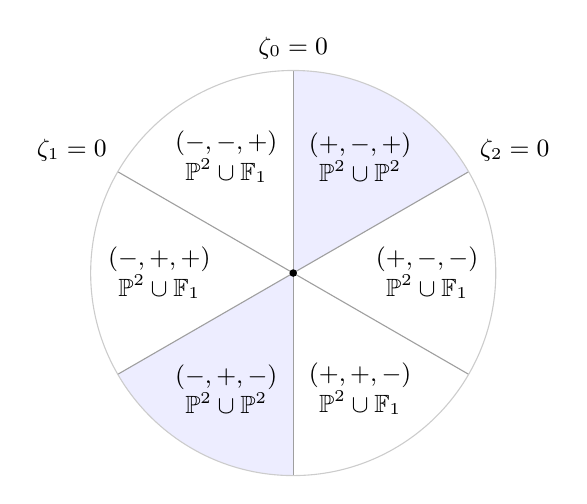
\begin{tikzpicture}[scale=1.05,font=\small]
 \fill[blue!7] (0,0)--(30:2.45) arc(30:90:2.45)--cycle;
 \fill[blue!7] (0,0)--(210:2.45) arc(210:270:2.45)--cycle;
 \foreach \angle in {30,90,150}
  {\draw[gray!75] (\angle:2.45)--(\angle+180:2.45);}
 \draw[gray!40] (0,0) circle[radius=2.45];
 \fill (0,0) circle[radius=1.3pt];
 \node[align=center] at (0:1.62) {$(+,-,-)$\\$\PP^2\cup\FF_1$};
 \node[align=center] at (60:1.62) {$(+,-,+)$\\$\PP^2\cup\PP^2$};
 \node[align=center] at (120:1.62) {$(-,-,+)$\\$\PP^2\cup\FF_1$};
 \node[align=center] at (180:1.62) {$(-,+,+)$\\$\PP^2\cup\FF_1$};
 \node[align=center] at (240:1.62) {$(-,+,-)$\\$\PP^2\cup\PP^2$};
 \node[align=center] at (300:1.62) {$(+,+,-)$\\$\PP^2\cup\FF_1$};
 \node[above] at (90:2.47) {$\zeta_0=0$};
 \node[above right] at (30:2.47) {$\zeta_2=0$};
 \node[above left] at (150:2.47) {$\zeta_1=0$};
\end{tikzpicture}

\end{adjustbox}
\caption{The six sectors in the moment parameter plane. Signs are
ordered $(\zeta_0,\zeta_1,\zeta_2)$. The shaded sectors have
two planes meeting at a point; in the other sectors the two
surfaces meet along a projective line.}
\label{fig:chambers}
\end{figure}

\subsection{Two planes and a reduced degeneration of curves}
Take $\zeta_0=a>0$, $\zeta_2=b>0$, and $\zeta_1=-a-b$.
Over the affine vertex every oriented-cycle invariant vanishes.
In particular,
\[
 zz'=ww'=0,\qquad u_i\varphi_j=0\quad(1\le i,j\le2).
\]
Thus $u=0$ or $\varphi=0$, and a nonzero triangle of
arrows must be acyclic. If $\varphi\ne0$, the positive
moment at vertex~2 forces $w\ne0$; the cycle equations
then force $z'=w'=0$. This component, including its
closure, is
\begin{equation}\label{eq:plane-zero-section}
 u=z'=w'=0,\qquad |z|^2+|\varphi|^2=a,\qquad
 |w|^2=b+|\varphi|^2.
\end{equation}
Eliminate the nonzero coordinate $w$ by complex gauge.
The remaining quotient is $[z:\varphi]\in\PP^2$.
Call it $P_0$: its objects have $L_0$ as subobject
and the spherical extension of $L_1,L_2$ as quotient.
The other component $P_2$ has $\varphi=z'=w'=0$,
$z\ne0$, and coordinates $[w:u]\in\PP^2$.
The components meet at the single point $p$ with
$u=\varphi=0$ and $z,w\ne0$.

These are all the components, since they exhaust the
acyclic supports. Near $p$ fix $z,w$ by complex gauge
and solve the two complex equations for $z',w'$.
The remaining smooth coordinates are $(u,\varphi)$.
Thus $P_0=\{u=0\}$ and $P_2=\{\varphi=0\}$ meet
transversely. The moving exceptional divisor $D$ is
locally $\varphi(u)=0$, with contraction to the
$A_1$ surface given by
\[
 A=u\otimes\varphi,\qquad \tr A=0.
\]
In particular, $D$ has an ordinary double point at $p$.
It is irreducible: its projective-line family over the
connected open surface $S^\circ$ is dense, and a
fibre over $o$ has dimension two, not three.

Fix nonzero $b_0\in\C^2$ and
$\beta_0\in(\C^2)^*$ with $\beta_0(b_0)=0$.
Over $A=t b_0\otimes\beta_0$, write
$u=\lambda b_0$, $\varphi=\nu\beta_0$,
$\lambda\nu=t$, and $z'=w'=0$. The compact
quotient has coordinates
\begin{equation}\label{eq:proper-specialization}
 [Z_0:Z_1]=[z:\nu w],\qquad
 [W_0:W_1]=[w:\lambda z],\qquad
 Z_1W_1=tZ_0W_0
\end{equation}
in $\PP^1\times\PP^1$. Stability makes each
homogeneous pair nonzero. On their four affine charts
the displayed expressions and the equation recover
the original quotient coordinates, including the
endpoints where $z$ or $w$ vanishes.

Equation~\eqref{eq:proper-specialization} is a relative
effective Cartier divisor of fixed bidegree $(1,1)$,
containing no entire ambient fibre. It is therefore
proper and flat over a disk. For $t\ne0$ its fibre
is $\PP^1$; for $t=0$ it is the reduced union of a
line in $P_0$ and a line in $P_2$. At their crossing
the equation is $xy=t$. Whole-fibre coverage from
Section~\ref{sec:compact-interaction} embeds this
compact family into the actual moduli space after
shrinking the disk. Consequently the specialization
maps in integral homology and fibre cohomology are
\begin{equation}\label{eq:reduced-specialization}
 H_2(\PP^1,\Z)\longrightarrow H_2(P_0\cup P_2,\Z),
 \quad 1\longmapsto(1,1),\qquad
 (n_0,n_2)\longmapsto n_0+n_2.
\end{equation}
This is a multiplicity-one geometric specialization,
not merely an identity of rational divisor pairings.

\begin{figure}[tb]
\centering
\begin{adjustbox}{max width=\textwidth}
% Schematic incidence, not a real-dimensional embedding of the complex surfaces.
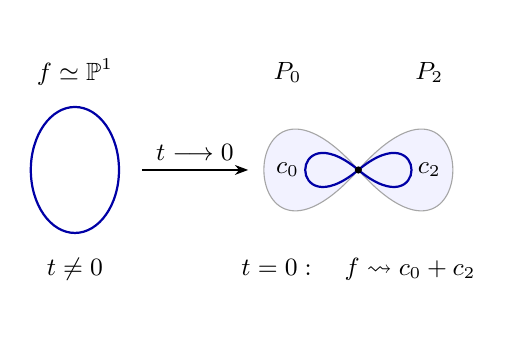
\begin{tikzpicture}[font=\small,>=Stealth]
 \draw[blue!65!black,thick] (-3.6,0) ellipse[x radius=.56,y radius=.8];
 \node[above] at (-3.6,.95) {$f\simeq\PP^1$};
 \node[below] at (-3.6,-1) {$t\ne0$};
 \draw[->] (-2.75,0)--(-1.4,0) node[midway,above] {$t\longrightarrow0$};
 \filldraw[fill=blue!5,draw=gray!70]
   (0,0) .. controls (-1.6,1.8) and (-1.6,-1.8) .. (0,0);
 \filldraw[fill=blue!5,draw=gray!70]
   (0,0) .. controls (1.6,1.8) and (1.6,-1.8) .. (0,0);
 \draw[blue!65!black,thick]
   (0,0) .. controls (-.9,.75) and (-.9,-.75) .. (0,0);
 \draw[blue!65!black,thick]
   (0,0) .. controls (.9,.75) and (.9,-.75) .. (0,0);
 \fill (0,0) circle[radius=1.3pt];
 \node[above] at (-.9,.99) {$P_0$};
 \node[above] at (.9,.99) {$P_2$};
 \node at (-.9,0) {$c_0$};
 \node at (.9,0) {$c_2$};
 \node[below] at (0,-1) {$t=0:\quad f\rightsquigarrow c_0+c_2$};
\end{tikzpicture}

\end{adjustbox}
\caption{Incidence schematic for the proper family
\eqref{eq:proper-specialization}. The marked curves in the two
planes each occur with multiplicity one; the local equation
at their common point is $xy=t$.}
\label{fig:specialization}
\end{figure}

\subsection{The other four chambers}
Two symmetries reduce the calculation to one more
sector. Interchanging every arrow with its paired
reverse and inverting the vertex bases identifies
the model at $\zeta$ with that at $-\zeta$.
The signed cotangent lift
\[
 (z,z',w,w',u,\varphi)\longmapsto
 (w,w',z,z',\varphi,-u)
\]
interchanges vertices 0 and 2. Both operations preserve
the complex zero equations and the flat metric.
They are symmetries of the finite models; they need
not arise from automorphisms of the fixed K3 surface.

Consider $\zeta_0=a>0$, $\zeta_1=b>0$,
$\zeta_2=-a-b$. A maximal acyclic support must use
the double edge in direction $2\to0$. The other
edges have one of the orientations $2\to1\to0$
or $2\to0\to1$. In the first case the coordinates
are $(\varphi,w',z)$ and
\[
 |\varphi|^2+|z|^2=a,\qquad |w'|^2-|z|^2=b.
\]
Eliminating the nonzero $w'$ leaves $\PP^2$.
In the second case they are $(\varphi,z',w')$ and
\[
 |\varphi|^2-|z'|^2=a,\qquad |z'|^2+|w'|^2=b.
\]
Here $\varphi\ne0$ and $(z',w')\ne0$. The
effective two-torus has weights $(1,0),(-1,1),(0,1)$
on these three groups of coordinates. The quotient
is the first Hirzebruch surface $\FF_1$: over
$[\varphi]\in\PP^1$ the coordinate $z'/w'$
transforms as a coordinate on $\OO_{\PP^1}(-1)$,
and its compactification adds the infinity section.

The two surfaces meet at $z=z'=0$, where
$\varphi,w'\ne0$. Their intersection is a line
in $\PP^2$ and the negative section in $\FF_1$.
For an explicit local check, fix
$\varphi=(1,q)$ and $w'=1$. The complex equations
give $u_1=zz'-qu_2$ and $w=-zz'$. In the smooth
coordinates $(z,z',u_2,q)$ the surfaces are
$\{z'=u_2=0\}$ and $\{z=u_2=0\}$.
Their intersection is clean, with tangent space
exactly the $q$-line; the second $\varphi$ chart
gives the same description at infinity.

We have proved the complete table
\begin{center}
\begin{adjustbox}{max width=\textwidth}
\begin{tabular}{lll}
\toprule
Signs of $(\zeta_0,\zeta_1,\zeta_2)$ & Components & Intersection\\
\midrule
$(+,-,+),\ (-,+,-)$ & $\PP^2,\ \PP^2$ & transverse point\\
$(+,+,-),\ (-,-,+)$ & $\PP^2,\ \FF_1$ & line / negative section\\
$(-,+,+),\ (+,-,-)$ & $\PP^2,\ \FF_1$ & line / negative section\\
\bottomrule
\end{tabular}
\end{adjustbox}
\end{center}
Each component is Lagrangian: its coordinate
subspace contains at most one direction from each
symplectically paired set of arrows, and has half
the dimension after reduction.

\subsection{Intersections and adjacent walls}
Write $P,R$ for the plane and ruled surface in the
second configuration. Their normal bundles are
$T^*P,T^*R$, giving self-intersections 3 and 4.
For their clean intersection $C\simeq\PP^1$ the
excess bundle is
$T_M/(T_P+T_R)|_C\simeq T^*C$, by the symplectic
form. The excess intersection formula gives
\begin{equation}\label{eq:ruled-intersections}
 P\cdot R=-2,\qquad
 B'=\begin{pmatrix}3&-2\\-2&4\end{pmatrix}.
\end{equation}
The negative sign comes from a curve of excess
intersection, rather than an isolated transverse
complex intersection.

Mayer--Vietoris for $P\cup_C R$ gives $H_0=\Z$
and $H_2=H_4=\Z^2$, with all other reduced homology
zero. The map from $H_2(C)$ is primitive because
its first component is a line. A regular neighborhood
$W$ retracts to this union. Poincar\'e--Lefschetz
duality identifies $H^4(W,\partial W)\to H^4(W)$
with $B'$. Its Smith invariants are $1,8$.
Thus the boundary groups are those in
\eqref{eq:two-plane-boundary} below, with quotient
functional $(n_P,n_R)\mapsto6n_P+n_R\pmod8$.
This is a calculation of the resolved-neighborhood
boundary. The global primitive embeddings used
in the next section are calculated in the two-plane
chamber.

Away from the origin, the walls $\zeta_0=0$ and
$\zeta_2=0$ have the doubled three-arrow
$\mathrm U(1)$ normal model. They contract an
isolated plane. The wall $\zeta_1=0$ has the
doubled two-arrow model and contracts the moving
projective-line family. Its normal singularity is
$A_1$. The factor classification and whole-fibre
coverage show that this list includes every
exceptional component in the chosen parameter
neighborhood.

\section{Integral cycles and their attachment}\label{sec:integral-attachments}

All cohomology in this section has integral coefficients
unless otherwise specified. The Mukai marking identifies
the exceptional curve classes, but rational intersection
formulas alone do not determine how their neighborhoods
attach to the complement. We calculate both the primitive
integral classes and the resulting boundary homomorphisms.

\subsection{Primitive classes in the isolated example}
On $P_+$ the universal extension has $K$-class
$b\,\OO(1)+a$, up to tensoring by a base line bundle.
For $x\in v^\perp$ this ambiguity disappears from
\eqref{eq:mukai-marking}; hence
\[
 \theta_+(x)|_{P_+}=(a,x)h,\qquad
 \theta_-(x)|_{P_-}=-(a,x)h.
\]
We identify a rational vector in $v^\perp$ with its
curve functional by the Mukai pairing. A plane line
therefore has class
\begin{equation}\label{eq:isolated-classes}
 \ell_\pm=\pm(a-v/2),\qquad q(\ell_\pm)=-5/2,
 \qquad \rho_\pm=\theta_\pm\bigl(\pm(2a-v)\bigr).
\end{equation}
The integral vector $w_0=(9,3D,-10)$ lies in $v^\perp$
and satisfies $(a,w_0)=1$. It proves that each line
is primitive. The vector $2a-v=(-1,-D,6)$ is primitive;
its pairings with $v^\perp$ are even, and its pairing
with $w_0$ is two. Thus $q(\rho_\pm)=-10$ and
$\rho_\pm$ has divisibility two. The restriction of
$\theta_\pm(w_0)^2$ to the plane is $h^2$, which
also proves primitivity of its surface class.

For a K3$^{[2]}$-type fourfold the polarized Fujiki
identities are
\begin{equation}\label{eq:fujiki}
 \begin{aligned}
 \int_M\alpha\beta\gamma\delta
 &=q(\alpha,\beta)q(\gamma,\delta)
   +q(\alpha,\gamma)q(\beta,\delta)
   +q(\alpha,\delta)q(\beta,\gamma),\\
 \int_M c_2(M)\alpha\beta&=30q(\alpha,\beta).
 \end{aligned}
\end{equation}
The rational map $\operatorname{Sym}^2H^2(M,\mathbb Q)
\to H^4(M,\mathbb Q)$ is an isomorphism. Since
$q(\ell)=-5/2$, the class $\ell^2/2+c_2(M)/24$
pairs with $\alpha\beta$ as
$q(\ell,\alpha)q(\ell,\beta)$, exactly the
restriction pairing on the plane. Nondegeneracy gives
the classical formula
\begin{equation}\label{eq:plane-class}
 [P_\pm]=\frac{\ell_\pm^2}{2}+\frac{c_2(M_\pm)}{24}
         =\frac{\rho_\pm^2}{8}+\frac{c_2(M_\pm)}{24}.
\end{equation}
See \cite{hassetttschinkel}, with the attribution
there to O'Grady. The cotangent normal bundle gives
$[P]^2=3$; from $T_M|_P=T_P+T^*_P$ in $K$-theory
one also gets $\int_Pc_2(M)=-3$. Formula
\eqref{eq:plane-class} is rational. The integral
primitivity assertion follows from $w_0$, without
assuming an integral symmetric-square presentation.

Totaro's torsion-freeness theorem
\cite[Theorem~3.1]{totaro} and the coefficient of
degree two in G\"ottsche's Hilbert-scheme formula
\cite{gottsche} give free even cohomology of ranks
$1,23,276,23,1$ for $M_\pm$. The contraction identifies
$Z$ homeomorphically with $M_\pm/P_\pm$: the map
from this compact quotient to the Hausdorff target
is bijective. The plane inclusion is a cofibration,
and its restrictions in degrees 0, 2 and 4 are
surjective. The pair sequence therefore gives
\begin{center}
\begin{adjustbox}{max width=\textwidth}
\begin{tabular}{lrrrrr}
\toprule
Space & $b_0$ & $b_2$ & $b_4$ & $b_6$ & $b_8$\\
\midrule
$M_\pm$ & 1&23&276&23&1\\
$Z$ &1&22&275&23&1\\
$M_\pm\setminus P_\pm$ &1&23&275&22&0\\
\bottomrule
\end{tabular}
\end{adjustbox}
\end{center}
All other groups vanish, and these groups are
torsion-free. The pullback from $Z$ is an injective
ring map whose image is
\begin{equation}\label{eq:isolated-target-ring}
 \Z\cdot1\ \oplus\left(\bigoplus_{k>0}
 \ker\bigl(H^k(M_\pm)\longrightarrow H^k(P_\pm)\bigr)\right).
\end{equation}
Its multiplication is inherited from the chamber
ring; the local singularity alone does not provide
that ring as additional output.

\subsection{The two interacting curve and surface classes}
Return to the chamber $\zeta_0,\zeta_2>0$, and put
$E=P_0\cup P_2$. Let $c_i$ be an effective line in
$P_i$ and $f$ a moving projective-line fibre. The
universal extensions on these fibres give
\begin{equation}\label{eq:interacting-curve-classes}
 \begin{gathered}
 l_i=a_i-v/2\quad(i=0,2),\qquad
 c_0=-l_0,\quad c_2=-l_2,\quad f=a_1,\\
 f=c_0+c_2,\qquad
 q(c_0)=q(c_2)=-5/2,\quad q(c_0,c_2)=3/2,\quad q(f)=-2.
 \end{gathered}
\end{equation}
Indeed the restriction to $P_i$ is
$\theta_v(x)|_{P_i}=-(a_i,x)h_i$. Over a moving
fibre the extension is $F\,\OO(1)+L_1$, so its
restriction is $-(w,x)h=(a_1,x)h$. This calculation
uses a fixed $F$ and needs no global ordinary
universal family on $S^\circ$. Equation
\eqref{eq:reduced-specialization} realizes the class
relation by a reduced family of actual curves.

Use the primitive lattice embedding
\eqref{eq:primitive-embedding}. The integral vectors
\[
 x=(0,f_2-f_3,0),\qquad y=(0,-3f_2,-1)
\]
are in $v^\perp$, with pairings $(0,1,-1)$ and
$(1,-2,1)$ against $(a_0,a_1,a_2)$.
The same witnesses exist for every primitive embedding of
$\NS(X)$: unimodularity of $H^2(X,\Z)$ makes the restriction
$H^2(X,\Z)\to\NS(X)^*$ surjective, so the prescribed
pairings of their degree-two components can always be realized.
For
$\alpha=\theta_v(x)$ and $\beta=\theta_v(y)$,
\begin{equation}\label{eq:restriction-witnesses}
 \alpha|_E=(0,h_2),\qquad \beta|_E=(-h_0,-h_2),
 \qquad
 \alpha^2|_E=(0,h_2^2),\quad
 \beta^2|_E=(h_0^2,h_2^2).
\end{equation}
Both restriction matrices are unimodular. Thus the
two line classes span a primitive subgroup of
$H_2(M)$, and the two plane classes span a primitive
subgroup of $H_4(M)$.

The cotangent normal bundles and the transverse
intersection at $p$ give
\begin{equation}\label{eq:two-plane-matrix}
 B=\begin{pmatrix}3&1\\1&3\end{pmatrix}.
\end{equation}
Equivalently, $[P_i]=l_i^2/2+c_2(M)/24$ by the
argument for \eqref{eq:plane-class}; the off-diagonal
intersection is $q(l_0,l_2)^2/2-1/8=1$.
Here the geometric intersection and the rational
Fujiki calculation agree, while
\eqref{eq:restriction-witnesses} supplies the integral
information.

\subsection{The neighborhood boundaries}
For one plane the boundary is the sphere bundle
$L=S(T^*\PP^2)$. Its Euler class is $3h^2$.
The Gysin sequence gives $H^j(L)=\Z$ for
$j=0,2,5,7$, $H^4(L)=\Z/3$, and zero otherwise.
In particular $H^3(L)=0$, although $H_3(L)=\Z/3$.

For two transverse planes take a closed regular
neighborhood $W$ with smoothed boundary $L$. It
is the plumbing of their normal disk bundles and
retracts to $E\simeq\PP^2\vee\PP^2$.
Poincar\'e--Lefschetz duality makes the middle map
$H^4(W,L)\to H^4(W)$ the matrix $B$.
The pair sequence, together with $\det B=8$ and
the gcd one of its entries, gives
\begin{equation}\label{eq:two-plane-boundary}
 H^j(L)=
 \begin{cases}
 \Z,&j=0,7,\\
 \Z^2,&j=2,5,\\
 \Z/8,&j=4,\\
 0,&\text{otherwise}.
 \end{cases}
\end{equation}
The quotient map on $H^4(W)=\Z^2$ is
\begin{equation}\label{eq:boundary-functional}
 (n_0,n_2)\longmapsto n_0-3n_2\pmod8.
\end{equation}
Its kernel is $B\Z^2$: it kills both columns and
is onto a group of order $\det B$.
This $L$ is a smooth boundary in the resolution.
The target has a positive-dimensional singular
stratum through $o$, so $L$ is not the link of an
isolated target singularity.

Alexander--Lefschetz duality gives
$H^k(M,M\setminus E)=H_{8-k}(E)$. The primitive
line, plane and point inclusions just proved show
that $V=M\setminus E$ has torsion-free even
cohomology, with ranks $1,23,274,21$ in degrees
$0,2,4,6$. In particular,
\begin{equation}\label{eq:complement-quotient}
 H^4(V)=H^4(M)/(\Z[P_0]+\Z[P_2]).
\end{equation}
Notice that $V$ retains the moving exceptional
divisor away from $E$.

\subsection{Calculated attachments on integral generators}
We now specify the map from the complement to the
boundary. The input includes the complement ring
with its distinguished universal-index classes.
The following formulas evaluate the attachment
without asking for an ambient lift of a given class.

For $z\in K^0_{\mathrm{top}}(X)$ define the family
index
\begin{equation}\label{eq:universal-index}
 I_z=p_{M!}\bigl(p_X^*(z^\vee)\otimes\cE\bigr)
       \in K^0_{\mathrm{top}}(M),\qquad
 \chi(F,z)=-(v(F),v(z)).
\end{equation}
Here $p_!$ is the complex $K$-theory pushforward.
Markman's integral-generation theorem
\cite[Theorem~1]{markman}, the integral K\"unneth
decomposition and the perfect Euler pairing on
$K^0_{\mathrm{top}}(X)$ show that the Chern classes
of these indices generate $H^*(M,\Z)$. Thus degree
four is generated by the classes $c_2(I_z)$ and
$c_1(I_z)c_1(I_{z'})$. Rational Chern characters
would not suffice for this conclusion.

One normalization removes the base-line ambiguity
of the universal family on the exceptional set.
For the isolated example, let $F,Q$ be its
subobject and quotient in the chosen chamber.
Their Mukai vectors span a primitive rank-two
sublattice: the rank-one factor and the primitive
$D$-coordinate give a unit minor. Unimodularity
supplies a topological class $y$ with
$\chi(F,y)=0$, $\chi(Q,y)=1$. On the plane
\[
 \cE=(F\,\OO(1)+Q)\otimes L,
 \qquad I_y|_P=L.
\]
The global index $I_y$ has rank one. Tensor
$\cE$ by $\det(I_y)^{-1}$ to remove $L$.
For this normalized topological universal class,
\begin{equation}\label{eq:isolated-index-restriction}
 c(I_z)|_P=(1+h)^{m_z},\qquad m_z=\chi(F,z).
\end{equation}
The powers are interpreted as total Chern classes
of virtual bundles and allow negative integers.

For the interacting planes the class
$y=(0,-f_2,0)$ has Euler pairings $(0,1,0)$ with
$(a_0,a_1,a_2)$. The same global determinant
normalization removes the line twists on \emph{both}
planes, including their common point. It gives
\begin{equation}\label{eq:interacting-index-restriction}
 c(I_z)|_{P_i}=(1+h_i)^{m_{i,z}},\qquad
 m_{i,z}=\chi(L_i,z),\quad i=0,2.
\end{equation}
This normalization is topological; it makes no
claim of an algebraic lift for the auxiliary
Brauer class considered in the next section.

\begin{proposition}\label{prop:calculated-attachments}
Let $A=H^*(V,\Z)$ be the complement ring with the
restrictions of the normalized index Chern classes
just specified.

For an isolated plane, the actual restriction
$\kappa:A^4\to H^4(L)=\Z/3$ is determined by
\begin{equation}\label{eq:mod-three-generators}
 \begin{aligned}
 \kappa(c_2(I_z)|_V)&=\binom{m_z}{2},\\
 \kappa(c_1(I_z)c_1(I_{z'})|_V)&=m_zm_{z'}
 \end{aligned}\qquad\pmod3,
\end{equation}
and restriction identifies
\begin{equation}\label{eq:mod-three-gluing}
 H^4(M)=\{(u,N)\in A^4\oplus\Z:
                      N\equiv\kappa(u)\pmod3\}.
\end{equation}
For the two-plane chamber, the actual restriction
$\kappa:A^4\to H^4(L)=\Z/8$ is determined by
\begin{equation}\label{eq:mod-eight-generators}
 \begin{aligned}
 \kappa(c_2(I_z)|_V)
   &=\binom{m_{0,z}}2-3\binom{m_{2,z}}2,\\
 \kappa(c_1(I_z)c_1(I_{z'})|_V)
   &=m_{0,z}m_{0,z'}-3m_{2,z}m_{2,z'}
 \end{aligned}\qquad\pmod8,
\end{equation}
and restriction identifies
\begin{equation}\label{eq:mod-eight-gluing}
 H^4(M)=\{(u,n_0,n_2)\in A^4\oplus\Z^2:
           n_0-3n_2\equiv\kappa(u)\pmod8\}.
\end{equation}
Both attachment maps are surjective.
\end{proposition}

\begin{proof}
The relative group $H^5(M,V)=H_3(E)$ vanishes
in both cases. Thus $H^4(M)\to A^4$ is onto,
and the restricted degree-four index monomials
generate $A^4$. Equations
\eqref{eq:isolated-index-restriction} and
\eqref{eq:interacting-index-restriction} give their
integer evaluations on the plane or planes.
Passing to the boundary gives exactly
\eqref{eq:mod-three-generators} and
\eqref{eq:mod-eight-generators}.

To check every relation among these generators,
let a degree-four integral polynomial in the
restricted Chern classes vanish on $V$. Its
ambient polynomial class lies in the relative
image $H^4(M,V)$, generated by the plane classes.
Its evaluations on $E$ therefore lie in
$3\Z$ or $B\Z^2$, respectively. The prescribed
boundary functional kills these subgroups.
Consequently the formulas are independent of the
chosen polynomial expression in $A^4$ and
define its actual boundary restriction.

Apply Mayer--Vietoris to $V$ and an open regular
neighborhood of $E$. Their overlap retracts to
$L$, and $H^3(L)=0$. The restriction from $M$
is therefore injective in degree four, with image
the kernel of the difference of the two boundary
maps. This is precisely the displayed fibre
product. Finally $\theta(w_0)^2$ evaluates to one
in the isolated case, while $\alpha^2$ evaluates
to $(0,1)$ in the interacting case. Their images
are units modulo three and eight.
\end{proof}

The construction retains the complement ring and
its marked index classes as input. It recovers
the integral degree-four attachment, including
the torsion boundary information that is absent
from Betti numbers. A change of index basis or
universal normalization changes the formulas for
the marked generators, but not the restriction
map they calculate.

\section{The projective-line family over the open stratum}\label{sec:projective-family}

Let $S\to T$ be the auxiliary K3 resolution, with
exceptional $(-2)$-curve $C$, and identify
$S^\circ=S\setminus C=T\setminus\{o\}$.
In the two-plane chamber write $D^\circ=D\setminus E$.
The map $\pi:D^\circ\to S^\circ$ is a projective-line
bundle. It has trivial monodromy on fibre cohomology,
yet a nonzero algebraic Brauer obstruction. This
distinction is visible in the global topology.

\subsection{Algebraic, analytic and topological lifts}
For a stable bundle $F$ of vector $w$, the groups
$\Hom(L_1,F)$ and $\Ext^2(L_1,F)$ vanish, while
$\dim\Ext^1(L_1,F)=2$. Local universal $w$-families
therefore give rank-two extension bundles. Their
projectivizations descend to $D^\circ$, with the
order-two Brauer class of the universal $w$-family.
This class remains nonzero on $S^\circ$: for a
regular integral scheme the Brauer group injects
into that of its function field
\cite[Corollaries~1.8 and~1.10]{grothendieckbrauer}.
Consequently $D^\circ$ has no presentation as the
projectivization of an ordinary \emph{algebraic}
rank-two vector bundle on $S^\circ$.

The curve $C$ is primitive in the unimodular K3
lattice, since its square is $-2$. The Gysin
sequence gives
\begin{equation}\label{eq:open-surface-cohomology}
 H^1(S^\circ)=H^3(S^\circ)=H^4(S^\circ)=0,
 \qquad H^2(S^\circ)=H^2(S)/\Z[C]\simeq\Z^{21}.
\end{equation}
The connected group $\mathrm{PGL}_2(\C)$ acts
trivially on $H^0(\PP^1)$ and $H^2(\PP^1)$.
The fibre cohomology local systems are thus
constant. There is also no topological obstruction
in degree three to lifting the projective bundle.
The class $u=\alpha|_{D^\circ}$ supplies an explicit
integral hyperplane class, because $\alpha\cdot f=1$.

An ordinary holomorphic lift exists as well. Siu's
top-degree coherent-cohomology theorem for a
connected noncompact complex manifold
\cite{siu} gives $H^2(S^\circ,\OO)=0$.
Together with $H^3(S^\circ,\Z)=0$, the exponential
sequence gives $H^2(S^\circ,\OO^*)=0$. The obstruction
from $1\to\OO^*\to\mathrm{GL}_2(\OO)
\to\mathrm{PGL}_2(\OO)\to1$ therefore vanishes.
There is no contradiction: on this nonproper
surface analytification need not retain an
algebraic Brauer obstruction.

\subsection{The divisor class, including its multiplicity}
We need the precise class of $D$ to calculate the
ring of $D^\circ$. Put $A=L_1$. The inequality
$\zeta_1<0$ means $\mu_\eta(A)>\mu_\eta(E)$,
so $\Hom(A,E)=0$ throughout the chamber.
Moreover $\chi(A,E)=-(a_1,v)=0$.

A nonzero map $E\to A$ has image
$A(-B)\otimes I_Z$ for an effective divisor $B$
and a zero-dimensional scheme $Z$. At $H$ its
image is a torsion-free quotient of a semistable
slope-zero bundle, so has nonnegative slope.
As a subsheaf of $A$ it has slope $-H\cdot B$.
Ampleness forces $B=0$. The kernel has slope zero
and is semistable. The complete factor and defect
classification of Lemma~\ref{lem:interacting-factor-list}
then forces $Z=\varnothing$ and makes the kernel
a bundle of vector $w$. Conversely the extension
fibres, including both deepest planes, have a
quotient to $A$. Hence $\Hom(E,A)\ne0$ precisely
on $D$.

The perfect complex $Rp_*R\Hom(A,\cE)$ has
amplitude $[1,2]$, virtual rank zero, and is
acyclic off $D$. Locally write it as
$K^1\xrightarrow{d}K^2$. Its determinant section
lies in $\det(K^1)^{-1}\otimes\det(K^2)$, whose
first Chern class is $\theta_v(a_1)$ by
Grothendieck--Riemann--Roch and
\eqref{eq:mukai-marking}.

We check that the section vanishes simply at a
generic point of $D$. There the bundle fits into
$0\to F\xrightarrow{j}E\xrightarrow{q}A\to0$,
with $F$ $H$-stable. The extension sequence,
$\Hom(F,A)=\Hom(A,F)=0$, and simplicity give
\[
 \begin{gathered}
 \Hom(F,E)=\C j,\quad \Hom(E,A)=\C q,\quad
 \Hom(E,E)=\C,\\
 \Ext^1(E,A)=\C,\quad
 \Ext^2(E,A)=0.
 \end{gathered}
\]
In the exact sequence
\[
 \Ext^1(E,E)\xrightarrow{q_*}\Ext^1(E,A)
 \longrightarrow\Ext^2(E,F)
 \xrightarrow{j_*}\Ext^2(E,E),
\]
the last arrow is an isomorphism: its Serre dual
sends $\operatorname{id}_E$ to $j$ between
one-dimensional spaces. Thus $q_*$ is onto.
For an infinitesimal deformation $\delta$ of $E$,
$q_*\delta$ is the obstruction to extending $q$.
Serre duality identifies this obstruction with
the first variation of the local differential
from $\Ext^1(A,E)$ to $\Ext^2(A,E)$, up to sign.
After cancelling acyclic summands, $d$ is a scalar
function with nonzero derivative. Its zero is
simple. These tangents preserve the determinant
because $H^1(X,\OO_X)=0$.

Since $D$ is irreducible and is the whole
divisorial support, we have proved
\begin{equation}\label{eq:divisor-class}
 [D]=\theta_v(a_1),\qquad D|_{P_i}=-h_i,
 \qquad D\cdot f=-2.
\end{equation}
The multiplicity argument is needed: the last
two intersection numbers by themselves would
not identify the global divisor class.

\subsection{The ring over the open stratum}
Use the integral isotropic Mukai map
$\theta_w:w^\perp/\Z w\to H^2(S,\Z)$ induced
by the same $w$-family as in the construction.
With $x$ from \eqref{eq:restriction-witnesses}, set
\[
 z=a_1+2x,\qquad d=\theta_w(z)|_{S^\circ}.
\]
Direct pairing gives $z\in v^\perp$,
$(z,a_1)=0$ and $(z,w)=0$. The universal
extension over $D^\circ$ gives
\begin{equation}\label{eq:mukai-open-compatibility}
 \theta_v(z)|_{D^\circ}=\pi^*\theta_w(z)|_{S^\circ}.
\end{equation}
Here is the descent argument for this global
identity. On the universal gerbe, use the
normalized rational Chern character of the
twisted family; equivalently divide the Chern
character of a quasi-universal family by its
similitude. Additivity in the universal extension
gives \eqref{eq:mukai-open-compatibility} in rational
cohomology. A tautological line, a base line or
a rational choice for the torsion gerbe affects
the degree-two pushforward only through
$(z,a_1)$, $(z,w)$ or $(z,v)$, all zero.
Thus the identity descends globally, rather
than only on contractible charts. Both sides
are integral. Leray--Hirsch with $u$ and
\eqref{eq:open-surface-cohomology} shows that
$H^2(D^\circ,\Z)$ is torsion-free, so the
rational equality is integral.

Combining it with \eqref{eq:divisor-class} gives
\begin{equation}\label{eq:relative-canonical}
 D|_{D^\circ}=-2u+\pi^*d.
\end{equation}
By adjunction this is the relative canonical
class: $M$ and $S^\circ$ have trivial canonical
bundles. Choose a topological rank-two lift $\mathcal W$
of the projective bundle, in the quotient
convention for $\PP(\mathcal W)$. Its hyperplane class
differs from $u$ by a pullback from the base.
Tensoring $\mathcal W$ with a topological line bundle
removes this difference. The normalized lift
has relative canonical class
$-2u+\pi^*c_1(\mathcal W)$, so injectivity of $\pi^*$
gives $c_1(\mathcal W)=d$. Also $c_2(\mathcal W)=0$ by
\eqref{eq:open-surface-cohomology}. The integral
projective-bundle formula now yields
\begin{equation}\label{eq:open-divisor-ring}
 H^*(D^\circ,\Z)
   =H^*(S^\circ,\Z)[u]/(u^2-du).
\end{equation}
This calculation specifies the hyperplane
normalization. It is consistent with the
nonzero algebraic Brauer class and the trivial
fibre-cohomology monodromy: these record
different aspects of the same family.

\section{Harmonic collapse and complete rescaled limits}\label{sec:harmonic-limits}

The classes calculated above determine exact periods.
To determine diameters, one must also compare paths
in the full compact moduli space. We first construct
compatible local comparisons and explain why short
ambient paths remain in them. This permits a relative
estimate even when one exceptional plane is much
smaller than the other.

\subsection{Exact periods of the reconstructed cycles}
Write
\[
 b_\eta=\left(0,[\omega_\eta],
       \frac{c_1(v)\cdot[\omega_\eta]}{\rank v}\right).
\]
Equation~\eqref{eq:harmonic-class} gives
$[\Omega_\eta]=2\pi^2\theta_v(b_\eta)$.
In the interacting family
$(a_i,b_\eta)=\deg_\eta L_i-\mu_\eta(v)
=-\zeta_i/(2\pi)$. Pairing with
\eqref{eq:interacting-curve-classes} proves
\begin{equation}\label{eq:exact-cycle-volumes}
 \begin{gathered}
 \operatorname{Area}(c_0)=\pi a,\qquad
 \operatorname{Area}(c_2)=\pi b,\qquad
 \operatorname{Area}(f)=\pi(a+b),\\
 \Vol(P_0)=\frac{(\pi a)^2}{2},\qquad
 \Vol(P_2)=\frac{(\pi b)^2}{2}.
 \end{gathered}
\end{equation}
The volume formula is $\int_P\Omega_\eta^2/2$.
These are exact identities for the actual harmonic
metric; they do not require its induced plane
metric to be Fubini--Study. The reduced
specialization of curves is reflected in exact
additivity of their areas.

For the isolated example put
$\kappa_t=44\pi|t|/3$. Its signed line class
\eqref{eq:isolated-classes} similarly gives
\begin{equation}\label{eq:isolated-periods}
 \operatorname{Area}(\ell_\pm)=\pi\kappa_t,
 \qquad \Vol(P_\pm)=\frac{(\pi\kappa_t)^2}{2}.
\end{equation}
The same $\kappa_t$ is the absolute moment level
in \eqref{eq:isolated-level}.

\subsection{Compatible comparisons over the entire exceptional set}
At the deeper point use the fixed background
$E_0=L_0\oplus L_1\oplus L_2$. Its chart
$\Phi_\eta$ has the full model
\eqref{eq:three-vertex-model} and the estimate
\eqref{eq:actual-quotient-comparison}, with radius
$r=\|x\|$. The common radius and constant are
independent of ratios of positive eigenvalues
of the orbit operator $C_x^*C_x$.
Section~\ref{sec:compact-interaction} proves that
the chart covers whole fibres and commutes with
the contraction to $Z$.

For $F$ in a compact subset of $S^\circ$, local
universal families give smoothly varying central
HE connections on $L_1\oplus F$. The elliptic
complement has a uniformly positive lower bound
on that compact set. Harmonic projections and
the finite-regularity estimates vary smoothly,
so finitely many charts have uniform constants.
Their full harmonic representations are
\begin{equation}\label{eq:moving-normal-model}
 U\oplus\bigl(\C^2\oplus(\C^2)^*\bigr),
 \qquad \dim_\C U=2,
 \qquad \kappa=2\pi(2\mu_\eta(v)-\deg_\eta F)=-\zeta_1.
\end{equation}
The effective group is a circle, trivial on $U$.
The factor two in the target comes from the rank
of $F$; the multiplicity-space moment still uses
ordinary trace.

Near $o$ these two-factor gaps need not remain
positive. Instead choose one fixed smaller
neighborhood of $o$ covered by the three-factor
chart. Its coverage includes moving fibres whose
base tends to $o$, by the normalized-map
compactness argument of
Section~\ref{sec:compact-interaction}. The
remaining part of the contracted locus is compact
in $S^\circ$ and admits the preceding finite cover.

On an overlap the transition is exactly
$h_{ij,\eta}=\Phi_{j,\eta}^{-1}\Phi_{i,\eta}$.
Both charts classify the same holomorphic
bundles; HE and finite balancing change their
presentations, not their isomorphism classes.
The transitions are holomorphic on the complex
quotient charts and commute with the contraction.
A base-line twist of a local universal family
does not change either assertion.
For $\varepsilon_i=C_i(|\eta|+r_i^2)<1/2$,
comparison with the same actual metric gives
\begin{equation}\label{eq:overlap-metric}
 \frac{1-\varepsilon_i}{1+\varepsilon_j}g_i
 \le h_{ij,\eta}^*g_j
 \le\frac{1+\varepsilon_i}{1-\varepsilon_j}g_i.
\end{equation}
This relative statement remains valid when
positive orbit eigenvalues become arbitrarily
small. A bound for ordinary derivatives of
balancing gauges is not required.

\subsection{From tensor comparison to ambient distances}
Equip each $\Q_\zeta$ with the length distance
$d_\zeta$ obtained from continuous paths which
are smooth in representation-type strata on a
finite subdivision, with finite one-sided
lengths at endpoints. The complex zero fibre
has the module-simple point
\eqref{eq:simple-point}. The finite intrinsic
metric theorem \cite[Section~5]{wuebben14}
therefore applies: these are proper geodesic
spaces with the compact quotient topology,
their distances vary continuously with balanced
representatives and levels, and every target
point is approximated at nearby levels.
The quotient norm radius is 1-Lipschitz.

Shrink the actual chart to have squared-metric
bounds $1/2$ and 2 on $r<2R$. Closed radial
sublevels are compact in the quotient and their
images are closed in the compact Hausdorff
moduli space. An actual path starting at radius
$r_0<R$ and leaving the radius-$R$ image must
pay at least
\begin{equation}\label{eq:first-exit}
 \frac{R-r_0}{\sqrt2}
\end{equation}
before its first exit. A segment of length $L$
remaining in the chart has radius at most
$r_0+\sqrt2L$. This applies to paths in the entire
moduli space and excludes a shortcut through
a distant part of that space.

Here is the resulting complete rescaling
statement, with its basepoint data made explicit.
Let $\eta_n\to0$ be generic, $\delta_n\downarrow0$,
and
\begin{equation}\label{eq:first-rescaling-data}
 \nu_n=\frac{\zeta(\eta_n)}{\delta_n^2}\longrightarrow\nu.
\end{equation}
Let $p_n$ be balanced representatives at levels
$\nu_n$ converging, after unitary adjustment,
to a representative $p$ at level $\nu$. Then
\begin{equation}\label{eq:first-rescaling-limit}
 \bigl(M_{\sigma(\eta_n)},\delta_n^{-1}d_{g_{\eta_n}},
       \Phi_{\eta_n}([\delta_np_n])\bigr)
 \longrightarrow(\Q_\nu,d_\nu,[p])
\end{equation}
in pointed Gromov--Hausdorff distance.

For completeness, homogeneity identifies the
current finite model with $\delta_n\Q_{\nu_n}$.
Finite near-minimizers on a bounded rescaled
ball have bounded radius, by its 1-Lipschitz
property, and scale into the actual chart.
Conversely an actual competitor of length
$O(\delta_n)$ cannot pay the fixed exit cost
\eqref{eq:first-exit}; its radius is
$O(\delta_n)$. Applying
\eqref{eq:actual-quotient-comparison} to both
types of competitors and taking both infima
gives relative distance error
\begin{equation}\label{eq:rescaled-relative-error}
 O_L(|\eta_n|+\delta_n^2)
\end{equation}
on each bounded rescaled ball. This comparison
also holds for pairs much closer than
$\delta_n$. The inverse chart covers every
actual bounded ball, and the model distance
continuity identifies the full complete target.
The estimate compares the actual metric with
the \emph{current} quotient $\Q_{\nu_n}$;
it does not prescribe a rate for
$\Q_{\nu_n}\to\Q_\nu$.

At a fixed point of $S^\circ$ the same proof
uses \eqref{eq:moving-normal-model}. It gives
the complete product of the flat harmonic
tangent space $U$ and the Eguchi--Hanson
quotient $T^*\PP^1$ at nonzero normalized level,
or $U\times(\C^2/\{\pm1\})$ at zero level.
The statements are uniform on compact subsets
of $S^\circ$.

\subsection{Two scales in the deepest fibre}
Let $C_i(a,b)$ denote the finite planes identified
with $P_i$, and put $\rho=a+b$. Their balanced
radii and finite ambient diameters are
$O(\sqrt\rho)$, by the finite core bound
\cite[Section~6]{wuebben14}. The preceding
first-exit argument, now at scale $\sqrt\rho$,
gives
\begin{equation}\label{eq:relative-plane-diameter}
 \diam_{g_\eta}P_i
  =\sqrt\rho\,(1+O(\rho))
        D_i(a/\rho,b/\rho),
\end{equation}
where $D_i(A,B)$ is the ambient diameter of
the indicated plane in the complete quotient
$\Q_{(A,-A-B,B)}$. The bounded inverse of the
linear parameter map makes $|\eta|=O(\rho)$
in this chamber. The error is relative even
when $D_i\to0$: shorter competitors stay in
the same radius-$O(\sqrt\rho)$ region, so no
division by a weak diameter occurs.

An explicit calculation separates the scales.
On $C_0$, use \eqref{eq:plane-zero-section} and
fix $w$ positive real. Before taking the
remaining common phase quotient of $(z,\varphi)$,
minimizing over the eliminated phase gives
\begin{equation}\label{eq:plane-metric-form}
 |dz|^2+|d\varphi|^2
 +\frac{(\operatorname{Re}\langle\varphi,d\varphi\rangle)^2}
             {b+|\varphi|^2}
 -\frac{(\operatorname{Im}\langle\varphi,d\varphi\rangle)^2}
             {b+2|\varphi|^2}.
\end{equation}
It lies between one half and twice the flat
form on $(z,\varphi)$. Infimizing over the
remaining phase preserves these inequalities.
Thus the induced plane metric is bounded
between one half and twice Fubini--Study at
line area $\pi a$. Its intrinsic diameter is
at most $\pi\sqrt a/\sqrt2$, an ambient upper
bound as well.

For a lower bound use the points with $z=0$,
$\varphi=\sqrt a(1,0)$ and $\sqrt a(0,1)$,
and $w=\sqrt{a+b}$. Any pair of their compact
group translates has Euclidean separation at
least $\sqrt{2a}$. Quotient length distance
dominates Euclidean orbit separation. Hence
\begin{equation}\label{eq:uniform-plane-bounds}
 \sqrt{2a}\le\diam_{d_\zeta}C_0(a,b)
       \le\frac\pi{\sqrt2}\sqrt a.
\end{equation}
Interchanging vertices gives the corresponding
bounds with $b$ for $C_2$. Combined with
\eqref{eq:relative-plane-diameter}, this proves
the ratio-independent bounds of
Theorem~\ref{thm:main}.

Suppose $a/b\to0$ and $\rho\to0$. After dividing
by $\sqrt b$, put $\epsilon=a/b$. The entire
plane satisfies
$|z|^2+|\varphi|^2=\epsilon$ and
$w=\sqrt{1+|\varphi|^2}=1+O(\epsilon)$.
It approaches the wall point $w=1$ uniformly.
Its stabilizer separates vertex~0 from the
spherical pair $(1,2)$. The full normal
representation has positive coordinates
$(z,\varphi_1,\varphi_2)$, their negative
duals, and effective level $\epsilon$.
There is no tangent factor. A second rescaling
by $\sqrt\epsilon$ gives the unit-level
Calabi quotient on $T^*\PP^2$, and the whole
plane converges to its zero section.

In that complete quotient
\[
 \{(q,p):p(q)=0,\ |q|^2-|p|^2=1\}/\mathrm U(1),
\]
the map $[q,p]\mapsto[q]$ is a retraction to
the zero section. Since $|q|\ge1$, its
Fubini--Study differential is bounded by the
ambient flat norm. Infimizing over vertical
directions makes it 1-Lipschitz on the
quotient. Ambient and intrinsic zero-section
distances therefore agree, and their diameter
is $\pi/2$. The relative comparisons at both
scales prove
\begin{equation}\label{eq:separated-diameter}
 \frac{\diam_{g_\eta}P_0}{\sqrt a}\longrightarrow\frac\pi2
       \quad(a/b\to0),
 \qquad
 \frac{\diam_{g_\eta}P_2}{\sqrt b}\longrightarrow\frac\pi2
       \quad(b/a\to0).
\end{equation}

\subsection{Successive complete limits}
The two-scale calculation is a particular case
of a statement with moving centers. The necessary
data include both the residual stability level
and the normal basepoint.

\begin{theorem}\label{thm:successive-limits}
Start with the actual rescaling
\eqref{eq:first-rescaling-data}--\eqref{eq:first-rescaling-limit}.
Let the current finite levels $\nu_n$ converge
to $\nu_*$ and the current basepoints converge
to $[x_*]\in\Q_{\nu_*}$. In the full normal
slice at $x_*$ write the representation as
$U\oplus W'$ with compact stabilizer $H$,
where $H$ acts trivially on $U$. Write the
balanced coordinates of the basepoints as
$(u_n,z_n)\to0$. Suppose $\sigma_n\downarrow0$ and
\begin{equation}\label{eq:successive-data}
 \frac{(\nu_n-\nu_*)|_{\Lie H}}{\sigma_n^2}
       \longrightarrow\lambda,
 \qquad \frac{z_n}{\sigma_n}\longrightarrow z_*
\end{equation}
after compact group adjustment. At physical
scale $\delta_n\sigma_n$ the complete pointed
limit is
\begin{equation}\label{eq:successive-product}
 U\times(W'///_\lambda H),\qquad (0,[z_*]).
\end{equation}
Here $///$ denotes the hyperk\"ahler quotient
with complex moment zero and real moment
$\lambda$. The statement may be iterated
through any fixed finite succession satisfying
\eqref{eq:successive-data} at each stage.
The physical scale is the product of the
successive scales. No bound on $|u_n|/\sigma_n$
is required.
\end{theorem}

\begin{proof}
The full normal-slice and moving-center
theorems \cite[Sections~4 and~6]{wuebben14}
give the comparison after the change
$(u,z)\mapsto(u_n+\sigma_nu,\sigma_nz)$.
On bounded normal balls its relative
squared-metric error is
\begin{equation}\label{eq:successive-error}
 O_{x_*}(|\nu_n-\nu_*|+|u_n|+\sigma_n R)=o(1).
\end{equation}
Translation removes the tangential motion
and does not change a moment level. The
outer error \eqref{eq:rescaled-relative-error}
is also multiplicative, so it adds to this
error and is not amplified by dividing by
$\sigma_n$.

Choose a fixed normal sublevel whose twice-sized
neighborhood lies in the slice. Its exit cost,
divided by $\sigma_n$, tends to infinity.
An actual path of length $O(\delta_n\sigma_n)$
therefore remains in both the outer chart and
the inner slice; its translated normal radius
is $O(\sigma_n)$. Conversely every bounded
normal-model near-minimizer maps into these
charts. Taking both length infima proves
relative distance comparison, and the common
inverse gives full ball coverage.

The existence of a module-simple point passes
to every full normal Ext representation
\cite[Section~6]{wuebben14}. Its finite metric
theorem applies to the full $U\oplus W'$;
the product decomposition then gives the
complete target \eqref{eq:successive-product}.
For finitely many stages the relative errors
sum to $o(1)$, and the successive exit estimates
and inverse charts give the asserted iteration.
Each limiting center has its own fixed radius
and constants. The statement requires the
convergent data at every stage and makes no
assertion about an infinite succession.
\end{proof}

For this quiver the nonzero $\zeta_0$ and
$\zeta_2$ walls have the isolated
$T^*\PP^2$ normal model. On a nonzero
$\zeta_1$ wall the tangent factor is $\C^2$
and the transverse model is $T^*\PP^1$.
If the internal scale in that pair-moduli
surface also vanishes, the same full normal
iteration applies. This describes approaches
from all six chambers without a lower bound
on a ratio of positive scales.

\subsection{The isolated and moving fibre constants}
In the isolated example the model plane is
the zero section of $T^*\PP^2$ at level
$\kappa_t$. Its induced metric is exactly
$\kappa_t g_{\rm FS}$, with line area $\pi\kappa_t$.
The actual comparison has error $O(|t|)$
on that entire section. The first-exit
argument and the 1-Lipschitz retraction give
\begin{equation}\label{eq:isolated-diameter}
 \diam_{g_t}P_\pm=\frac\pi2\sqrt{\kappa_t}
                       (1+O(|t|)).
\end{equation}
Dividing distances by $\sqrt{\kappa_t}$ gives
the complete unit Calabi quotient, with the
zero section as the limit of the actual plane.

For a moving fibre $F_y$ over $y\in S^\circ$,
the same argument in the two-arrow model
gives
\begin{equation}\label{eq:moving-diameter}
 \operatorname{Area}(F_y)=\pi|\zeta_1|,
 \qquad
 \frac{\diam_{g_\eta}F_y}{\sqrt{|\zeta_1|}}
       \longrightarrow\frac\pi2.
\end{equation}
The limit is through nonzero transverse
levels as $\eta\to0$, uniformly for $y$
in a compact subset of $S^\circ$.
The complete normal limit is Eguchi--Hanson
times the harmonic tangent plane. When
$y\to o$, the fixed three-factor chart and
the retained rescaled basepoint supply the
applicable limit instead. These are the
same fibres that specialize in
\eqref{eq:proper-specialization}.

\section{The compact harmonic limit}\label{sec:global-completion}

The local estimates identify the geometry near the
exceptional cycles. We finish by identifying the
completion of the regular harmonic metric and the
limit of the entire compact spaces. In the isolated
example a direct collapsing-neighborhood argument
suffices. For the interacting family we identify
the limiting semiample class and apply the
Ricci-flat degeneration theorems of Tosatti and
Song to the actual harmonic metrics.

\subsection{Smooth convergence on the stable open set}
Let $U=Z_{\rm reg}$, identified with the
$H$-stable bundle locus, and write $g_0$ for its
central harmonic metric. A compact subset of
$U$ is covered by finitely many local universal
families. At each central bundle the normalized
fixed-determinant HE equation has invertible
trace-free gauge linearization, since stability
removes its kernel. Compactness supplies a
uniform positive lower bound. The parameter
implicit-function theorem and elliptic
bootstrapping give smooth variation of the
normalized HE metrics. The deformation kernels
have constant dimension on this smooth locus,
so their harmonic projections vary smoothly
as well. Consequently
\begin{equation}\label{eq:regular-smooth-limit}
 g_\eta\longrightarrow g_0
 \quad\text{in every fixed }C^k\text{ norm on compact subsets of }U.
\end{equation}
These are the same holomorphic bundles in every
nearby chamber. The identification is the
restriction of the classifying contraction.

\subsection{A direct argument for the isolated plane}
In the isolated zero-level model, distance to
the cone vertex is the norm radius. The local
harmonic comparison shows that a radius-$\rho$
neighborhood has diameter $O(\rho)$ and that
adding the vertex is exactly the local metric
completion, with its quotient topology.
Outside such a neighborhood the target is
compact and smooth. Thus the completion of
$(U,g_0)$ is $Z$, with no further end.

One can also see compact convergence directly.
Use the invariant $A=u\otimes\varphi$ from
\eqref{eq:isolated-incidence}, and take the
target neighborhood where its nonzero singular
value is at most $\rho^2/2$. In the balanced
model, if $\kappa_t\le\rho^2$, its whole
preimage has radius $O(\rho)$ and diameter
$O(\rho)$, uniformly in $t$. Whole-fibre
coverage and the ambient comparison transfer
this bound to the actual moduli space.

Collapse each of these neighborhoods to a
point. A shortest quotient path needs to
visit that point at most once; lifting the
visit across a set of diameter $O(\rho)$
changes distance by at most $O(\rho)$.
For fixed $\rho$, the common compact exterior
has smoothly convergent metrics by
\eqref{eq:regular-smooth-limit}, so the
collapsed spaces converge in length distance.
The limsup of the original compact
Gromov--Hausdorff distance is therefore at
most $C\rho$. Letting $\rho\downarrow0$
proves convergence to the central completion.

\subsection{The limiting class gives the actual contraction}
In the interacting example put $c=D_1+D_2$
and $b_0=(0,H,0)\in v^\perp$. On every
chamber,
\[
 \frac{[\Omega_\eta]}{2\pi^2}
       \longrightarrow\theta_v(b_0).
\]
To identify this limiting class globally, use
the Greb--Toma determinant construction with
a sufficiently large very ample multiple $mH$.
Its surface $K$-class is
\[
 u_1=-3[\OO_{mH}]
       +\chi(E\otimes\OO_{mH})[\OO_x].
\]
Riemann--Roch gives
\[
 v(\OO_{mH})=(0,mH,-(mH)^2/2),\qquad
 v(u_1)=(0,-3mH,c\cdot mH).
\]
Their determinant convention is
$\lambda_{\cE}(u_1)=\det Rp_*(\cE\otimes p_X^*u_1)$
\cite[Definition~2.1]{grebtoma}. Since our
Mukai convention inserts the dual vector,
and $c\cdot H=0$, we obtain
\begin{equation}\label{eq:determinant-polarization}
 c_1\lambda_{\cE}(u_1)=3m\theta_v(b_0).
\end{equation}

The classifying theorem gives an ample line
on the slope target whose pullback is
$\lambda_{\cE}(u_1)^N$ for a positive integer
$N$. Restrict to the common reduced image
and pull back under its finite normalization.
The resulting line $A_Z$ on $Z$ is ample.
Using a common power for the finitely many
chambers gives
\begin{equation}\label{eq:common-ample-class}
 \theta_v(b_0)=\pi_\sigma^*\alpha_Z,
 \qquad \alpha_Z=\frac{c_1(A_Z)}{3mN}.
\end{equation}
The maps here are precisely the classifying
contractions already constructed. Thus the
limiting class is big and nef, and its
sufficiently divisible multiples define
this connected-fibre semiample morphism.
Vanishing on the named exceptional curves
alone would not have identified the ample
class on the target.

\subsection{Ricci-flatness and metric identification}
Every chamber object is locally free and
slope stable. At fixed determinant its
trace-free HE connection is an irreducible
projective ASD connection on the Ricci-flat
K3 surface. Itoh's construction
\cite[Theorem~2.1]{itoh} makes its smooth
moduli metric hyperk\"ahler. The real
Dolbeault metric differs by the fixed factor
specified in Section~\ref{sec:harmonic-models};
it is therefore hyperk\"ahler as well,
smooth on the entire compact $M_\sigma$,
and complete. By uniqueness in a K\"ahler
class,
$g_\eta/(2\pi^2)$ is the Ricci-flat metric
in class $\theta_v(b_\eta)$ on that fixed
complex manifold. No auxiliary metric on
a deformation-equivalent space is used.

The symplectic form on $U$ pulls back and
extends as the symplectic form on
$M_\sigma$. Its top power trivializes the
canonical sheaf on $U$. Normality and the
codimension-at-least-two singular complement
give the trivial reflexive canonical sheaf
on $Z$. The resolution has zero discrepancies;
further resolutions have nonnegative
discrepancies, since $M_\sigma$ is smooth.
Hence $Z$ is a projective Calabi--Yau
variety with canonical singularities and
a crepant resolution, as required by the
metric completion results.

Tosatti's real-class degeneration theorem
\cite[Theorem~1.1 and the subsequent sequence
formulation]{tosatti} applies to
$\theta_v(b_\eta)\to\pi_\sigma^*\alpha_Z$.
Its smooth limit away from the exceptional
locus is the regular Ricci-flat metric
of $\alpha_Z$ on $Z$. Equation
\eqref{eq:regular-smooth-limit} identifies
that metric with $g_0/(2\pi^2)$.
This equality of metric tensors is a separate
step from the algebraic/Uhlenbeck topological
identification.

\begin{proposition}\label{prop:compact-limit}
The completion of $(U,g_0)$ is a compact
length space $(Z,d_0)$ whose topology is
the projective topology. For every generic
sequence $\eta\to0$, allowing changes of
chamber and arbitrary ratios of its positive
scales,
\[
 (M_{\sigma(\eta)},g_\eta)
          \longrightarrow(Z,d_0)
 \quad\text{in compact Gromov--Hausdorff distance}.
\]
\end{proposition}

\begin{proof}
Song's completion theorem
\cite[Theorem~1.1]{song} applies to
$(Z,\alpha_Z)$. Its regular Ricci-flat
metric has compact completion homeomorphic
to $Z$, extending the identity on $U$.
The metric identification above and a fixed
homothety give the first assertion.
On a fixed chamber, \cite[Corollary~1.1]{song}
gives compact convergence of the Ricci-flat
metrics to that completion. Its limiting
class is rational, big and nef, with
semiample model exactly $Z$ by
\eqref{eq:common-ample-class}.

The conclusion applies to real interior
classes as well. If rational approximants
are used in this argument, approximate the
$n$th interior metric by a rational interior
class with Gromov--Hausdorff discrepancy
less than $1/n$. Smooth dependence at each
interior class permits this choice, and the
approximating classes still tend to the
same boundary class. No continuity estimate
uniform up to the boundary is assumed.

There are only six chambers. Every generic
parameter sequence has subsequences in a
single chamber. The determinant calculation
and the regular harmonic identification
give the same $(Z,d_0)$ for all such
subsequences. The subsequence criterion
proves the assertion for the original
sequence.
\end{proof}

\begin{proof}[Proof of Theorem~\ref{thm:main}]
Section~\ref{sec:compact-interaction} constructs
the compact chamber spaces, excludes all
ideal charge and identifies the full
singular locus of their common normal
target. Section~\ref{sec:chambers} gives
all six deepest fibres and the reduced
specialization. The primitive cycle
calculations and Proposition
\ref{prop:calculated-attachments} prove
the integral assertions. Equations
\eqref{eq:exact-cycle-volumes},
\eqref{eq:relative-plane-diameter},
\eqref{eq:uniform-plane-bounds} and
\eqref{eq:separated-diameter}, together
with Theorem~\ref{thm:successive-limits},
give the exact periods, ambient collapse
and complete rescaled limits for those
same cycles. Proposition~\ref{prop:compact-limit}
proves the final compact convergence.
\end{proof}

The integral attachment uses a marked
complement, and the metric completion uses
the global harmonic class on the actual
compact family. The exceptional cycles
thus carry explicit global information,
while the geometry retained away from
them remains part of the reconstruction
data. The argument concerns these
contractions without lost charge. Extending
it to singular graded sheaves and bubbling
would require compatible local metrics and
integral attachment data for those additional
boundary strata.

\begin{thebibliography}{Wue26b}

\bibitem[AS18]{arbarellosacca}
E. Arbarello and G. Sacc\`a,
\emph{Singularities of moduli spaces of sheaves on K3 surfaces and
Nakajima quiver varieties}, Adv. Math. \textbf{329} (2018), 649--703.
\href{https://doi.org/10.1016/j.aim.2018.02.003}{doi:10.1016/j.aim.2018.02.003}.

\bibitem[BMM21]{bmm}
R. Bandiera, M. Manetti and F. Meazzini,
\emph{Formality conjecture for minimal surfaces of Kodaira dimension 0},
Compos. Math. \textbf{157} (2021), 215--235.
\href{https://doi.org/10.1112/S0010437X20007605}{doi:10.1112/S0010437X20007605}.

\bibitem[BM14]{bayermacri}
A. Bayer and E. Macr\`i,
\emph{MMP for moduli of sheaves on K3s via wall-crossing: nef and
movable cones, Lagrangian fibrations}, Invent. Math. \textbf{198}
(2014), 505--590.
\href{https://doi.org/10.1007/s00222-014-0501-8}{doi:10.1007/s00222-014-0501-8}.

\bibitem[BD00]{bielawskidancer}
R. Bielawski and A. S. Dancer,
\emph{The geometry and topology of toric hyperk\"ahler manifolds},
Comm. Anal. Geom. \textbf{8} (2000), no.~4, 727--759.
\href{https://doi.org/10.4310/CAG.2000.v8.n4.a2}{doi:10.4310/CAG.2000.v8.n4.a2}.

\bibitem[BS16]{biswasschumacher}
I. Biswas and G. Schumacher,
\emph{The Weil-Petersson current for moduli of vector bundles and
applications to orbifolds}, Ann. Fac. Sci. Toulouse Math. (6)
\textbf{25} (2016), no.~4, 895--917.
\href{https://doi.org/10.5802/afst.1514}{doi:10.5802/afst.1514}.

\bibitem[Cal02]{caldararu}
A. C\u{a}ld\u{a}raru,
\emph{Non-fine moduli spaces of sheaves on K3 surfaces},
Internat. Math. Res. Notices \textbf{2002}, no.~20, 1027--1056.
\href{https://doi.org/10.1155/S1073792802109093}{doi:10.1155/S1073792802109093}.

\bibitem[G\"ot90]{gottsche}
L. G\"ottsche,
\emph{The Betti numbers of the Hilbert scheme of points on a smooth
projective surface}, Math. Ann. \textbf{286} (1990), 193--207.
\href{https://doi.org/10.1007/BF01453572}{doi:10.1007/BF01453572}.

\bibitem[GSTW21]{gstw}
D. Greb, B. Sibley, M. Toma and R. Wentworth,
\emph{Complex algebraic compactifications of the moduli space of
Hermitian--Yang--Mills connections on a projective manifold},
Geom. Topol. \textbf{25} (2021), 1719--1818.
\href{https://doi.org/10.2140/gt.2021.25.1719}{doi:10.2140/gt.2021.25.1719}.

\bibitem[GT17]{grebtoma}
D. Greb and M. Toma,
\emph{Compact moduli spaces for slope-semistable sheaves},
Algebr. Geom. \textbf{4} (2017), no.~1, 40--78.
\href{https://doi.org/10.14231/AG-2017-003}{doi:10.14231/AG-2017-003}.

\bibitem[Gro66]{grothendieckbrauer}
A. Grothendieck,
\emph{Le groupe de Brauer: II. Th\'eories cohomologiques},
S\'eminaire Bourbaki, ann\'ees 1964/65--1965/66, no.~9,
Soci\'et\'e math\'ematique de France, 1966, expos\'e~297, 287--307.
\href{https://numdam.org/item/SB_1964-1966__9__287_0/}{Numdam: SB\_1964-1966\_\_9\_\_287\_0}.

\bibitem[HT09]{hassetttschinkel}
B. Hassett and Y. Tschinkel,
\emph{Moving and ample cones of holomorphic symplectic fourfolds},
Geom. Funct. Anal. \textbf{19} (2009), 1065--1080.
\href{https://doi.org/10.1007/s00039-009-0022-6}{doi:10.1007/s00039-009-0022-6}.

\bibitem[HL10]{huybrechtslehn}
D. Huybrechts and M. Lehn,
\emph{The Geometry of Moduli Spaces of Sheaves}, 2nd ed.,
Cambridge Mathematical Library, Cambridge University Press,
Cambridge, 2010.
\href{https://doi.org/10.1017/CBO9780511711985}{doi:10.1017/CBO9780511711985}.

\bibitem[Ito88]{itoh}
M. Itoh,
\emph{Gauge fields and quaternion structure},
Kodai Math. J. \textbf{11} (1988), no.~3, 344--360.
\href{https://doi.org/10.2996/kmj/1138038932}{doi:10.2996/kmj/1138038932}.

\bibitem[Mar07]{markman}
E. Markman,
\emph{Integral generators for the cohomology ring of moduli spaces
of sheaves over Poisson surfaces}, Adv. Math. \textbf{208} (2007),
no.~2, 622--646.
\href{https://doi.org/10.1016/j.aim.2006.03.006}{doi:10.1016/j.aim.2006.03.006}.

\bibitem[MO23]{meazzinionorati}
F. Meazzini and C. Onorati,
\emph{Hyper-holomorphic connections on vector bundles on hyper-K\"ahler
manifolds}, Math. Z. \textbf{303} (2023), no.~1, article~17.
\href{https://doi.org/10.1007/s00209-022-03176-4}{doi:10.1007/s00209-022-03176-4}.

\bibitem[Mor84]{morrison}
D. R. Morrison,
\emph{On K3 surfaces with large Picard number},
Invent. Math. \textbf{75} (1984), 105--121.
\href{https://doi.org/10.1007/BF01403093}{doi:10.1007/BF01403093}.

\bibitem[Siu69]{siu}
Y.-T. Siu,
\emph{Analytic sheaf cohomology groups of dimension $n$ of
$n$-dimensional noncompact complex manifolds},
Pacific J. Math. \textbf{28} (1969), no.~2, 407--411.
\href{https://doi.org/10.2140/pjm.1969.28.407}{doi:10.2140/pjm.1969.28.407}.

\bibitem[Son14]{song}
J. Song,
\emph{Riemannian geometry of K\"ahler--Einstein currents},
preprint, 2014.
\href{https://arxiv.org/abs/1404.0445}{arXiv:1404.0445}.

\bibitem[Tos09]{tosatti}
V. Tosatti,
\emph{Limits of Calabi--Yau metrics when the K\"ahler class degenerates},
J. Eur. Math. Soc. (JEMS) \textbf{11} (2009), no.~4, 755--776.
\href{https://doi.org/10.4171/JEMS/165}{doi:10.4171/JEMS/165}.

\bibitem[Tot20]{totaro}
B. Totaro,
\emph{The integral cohomology of the Hilbert scheme of points on a surface},
Forum Math. Sigma \textbf{8} (2020), article~e40.
\href{https://doi.org/10.1017/fms.2020.35}{doi:10.1017/fms.2020.35}.

\bibitem[Weh04]{wehrheim}
K. Wehrheim,
\emph{Uhlenbeck Compactness}, EMS Series of Lectures in Mathematics,
European Mathematical Society, Z\"urich, 2004.
\href{https://doi.org/10.4171/004}{doi:10.4171/004}.

\bibitem[Wue26a]{wuebben14}
B. J. Wuebben,
\emph{Quantitative metric wall crossing for K3 bundle moduli},
6 November 2026.
\href{https://doi.org/10.5281/zenodo.24024998}{doi:10.5281/zenodo.24024998}.

\bibitem[Wue26b]{wuebben15}
B. J. Wuebben,
\emph{Quantitative local models for Hermitian--Einstein metrics},
7 November 2026.
\href{https://doi.org/10.5281/zenodo.24029090}{doi:10.5281/zenodo.24029090}.

\bibitem[Yos00]{yoshioka99}
K. Yoshioka,
\emph{Irreducibility of moduli spaces of vector bundles on K3 surfaces},
preprint, 2000.
\href{https://arxiv.org/abs/math/9907001v2}{arXiv:math/9907001v2}.

\bibitem[Yos01]{yoshioka01}
K. Yoshioka,
\emph{Moduli spaces of stable sheaves on abelian surfaces},
Math. Ann. \textbf{321} (2001), 817--884.
\href{https://doi.org/10.1007/s002080100255}{doi:10.1007/s002080100255}.

\end{thebibliography}

\bigskip
\noindent{\sc Bernd Johannes Wuebben, New York, NY,}
\texttt{wuebben@gmail.com}
\end{document}

